\documentclass[journal]{IEEEtran}

\usepackage{graphicx}
\usepackage{booktabs}
\usepackage{amsmath}
\usepackage{array}
\usepackage{cite}
\usepackage{url}
\usepackage{xcolor}
\usepackage{subcaption}
\usepackage[hidelinks]{hyperref}

\usepackage{tikz}
\usetikzlibrary{positioning,arrows.meta,calc,shapes.geometric,fit}

% ---------------------------------------------------------------------------
% Design tokens carried over from the Google Stitch mock-up, so the diagrams
% and the deployed interface share one palette.
% ---------------------------------------------------------------------------
\definecolor{stitchcyan}{HTML}{00E5FF}
\definecolor{stitchink}{HTML}{0B0E13}
\definecolor{stitchpanel}{HTML}{161A22}
\definecolor{stitchviolet}{HTML}{B39DDB}
\definecolor{stitchamber}{HTML}{FFCA58}
\definecolor{stitchcoral}{HTML}{FF7D7D}
\definecolor{stitchgreen}{HTML}{69F0AE}
\definecolor{stitchmute}{HTML}{8A93A6}
\definecolor{stitchgrid}{HTML}{3C4457}

\graphicspath{{figs/}{../restoration/results/}{../task4/results/}{../}}

\urlstyle{same}

\newcommand{\taskname}[1]{\textsc{#1}}

\begin{document}

\title{A Four-Task Generative Suite for Image Restoration and Sketch Synthesis:\\
Architecture Search, Soft Expert Routing, and Browser Deployment}

\author{GenAI~Assignment~\#1%
\thanks{Source code: \url{https://github.com/abdullahamin231/genai-assignment-1}}%
\thanks{Walkthrough video (5--7~minutes): \url{https://youtu.be/8YehNdrgRhQ}.}}

\markboth{Generative AI --- Assignment \#1}{%
Generative AI --- Assignment \#1: Four-Task Generative Image Restoration Suite}

\maketitle

\begin{abstract}
This paper presents the design, training, evaluation, and deployment of four related generative models that form a single browser-based image tool. The first three tasks address image restoration of $128\times128$ photographs corrupted by salt-and-pepper noise, Gaussian blur, and rectangular occlusion: a plain convolutional autoencoder that restores any input without knowing what is wrong with it (\taskname{Task~1}); a corruption classifier that identifies the degradation and routes the image to one of three specialist autoencoders through an explicit hard switch (\taskname{Task~2}); and a soft mixture-of-experts model whose gating network blends the identity path and all three specialists with temperature-scaled softmax weights (\taskname{Task~3}). The fourth task is a conditional GAN that translates facial photographs into pencil sketches in one of three artist styles (\taskname{Task~4}). Every architecture, loss function, and hyperparameter range was investigated against published alternatives before selection, and each task was tuned with Optuna under median-pruned asynchronous successive halving (14--30 trials per study, 44--60\% of trials pruned). On the official test split the autoencoder reaches 0.777 overall SSIM against 0.681 for the corrupted input; the classifier attains 99.77\% accuracy and 0.996 macro-F1, misrouting only 86 of 36{,}690 images; the soft mixture-of-experts improves aggregate SSIM to 0.841 over 0.817 for hard routing while raising gate accuracy to 83.99\%; and the sketch generator attains 0.510 SSIM against its paired targets. The four models are exported to ONNX and served by a FastAPI backend behind an nginx reverse proxy, packaged with Docker Compose so the entire system runs from a single documented command. Every figure, table, and architecture diagram in this paper is interpreted in the surrounding text.
\end{abstract}

\begin{IEEEkeywords}
image restoration, mixture-of-experts, conditional GAN, autoencoder, hyperparameter optimization, ONNX, web deployment
\end{IEEEkeywords}

\IEEEpeerreviewmaketitle

% ===========================================================================
\section{Introduction}
\label{sec:intro}
% ===========================================================================

Digital images arrive damaged. A photograph may be speckled by impulse noise, smeared by motion or defocus blur, or have a region occluded by an overlay; a different application may want the same photograph redrawn as a pencil sketch. These are not four unrelated problems. Salt-and-pepper noise, blur, and occlusion are all instance-level degradations of a single latent clean image, and photograph-to-sketch translation is a paired re-rendering of a single latent semantic content. Treating them as one suite therefore lets shared machinery --- a common $128\times128$ RGB interface, a shared corruption library, one exported-weights deployment path --- carry across all four systems.

The assignment asks for a deliberate progression in how a model decides \emph{what} to do to an image. A plain autoencoder cannot decide anything: it applies one fixed mapping to every input, which is exactly the right baseline and the right thing to measure against. A classifier plus specialists makes the decision discrete and inspectable: an argmax over four logits selects exactly one of four computation paths, and the selection is reported to the user as a confidence. A soft mixture-of-experts replaces that discrete decision with a differentiable convex combination, so ambiguous or compound degradations can be shared across specialists rather than forced onto one. Finally, a conditional GAN leaves restoration entirely and performs paired image-to-image translation, where an adversarial objective rather than a pixel distance defines quality.

This paper reports the full investigation: the literature and documentation consulted for each design decision (\S\ref{sec:related}), how the datasets were assembled and exactly which corruption parameters were applied (\S\ref{sec:data}), the four architectures and the alternatives rejected (\S\ref{sec:arch}), the loss functions and why each weighting was chosen (\S\ref{sec:loss}), the training procedure including staged and joint schedules (\S\ref{sec:train}), the Optuna search spaces and pruning strategy (\S\ref{sec:optuna}), the experimental setup (\S\ref{sec:setup}), the results with per-figure analysis (\S\ref{sec:results}), the deployed application architecture (\S\ref{sec:app}), the limitations observed (\S\ref{sec:limits}), and conclusions (\S\ref{sec:concl}). An appendix documents the AI assistance used (\S\ref{sec:ai}).

The paper's contributions are: (i)~an empirical comparison of three routing regimes --- none, hard, and soft --- on an identical corruption suite and test split, quantifying the gain from discreteness to differentiability; (ii)~four independently tuned architectures whose hyperparameters were selected by a consistent pruned-search protocol rather than by hand; and (iii)~a reproducible single-command deployment that serves all four models from ONNX exports behind one HTTP API.

% ===========================================================================
\section{Related Research}
\label{sec:related}
% ===========================================================================

\subsection{Restoration with plain autoencoders}

Convolutional autoencoders learn a bottleneck representation and reconstruct from it alone. The absence of skip connections is a deliberate constraint: U-Net~\cite{ronneberger2015unet} and encoder--decoder designs with lateral connections can copy high-frequency detail from input to output, which would let an identity shortcut masquerade as restoration. We wanted Task~1 to be measured honestly on how much the bottleneck itself recovers, so the model in \S\ref{sec:arch1} has no skip connections at all and is penalised if it degenerates to copying. Pixel-space $L_1$ was chosen over $L_2$ because $L_2$ over-penalises large residuals and produces blurrier regressions; this is the standard argument for $L_1$ in restoration losses~\cite{mathieu2016disentangling,isola2017pix2pix}. SSIM~\cite{wang2004image} is combined with $L_1$ rather than substituted for it, because SSIM alone is insensitive to the small systematic biases that $L_1$ pins down.

\subsection{Choosing a degradation: classifier and specialists}

The alternative to a single restoration network is to first \emph{identify} the degradation. This is the premise of all-in-one restoration, where a shared backbone is conditioned on an estimated degradation descriptor~\cite{zamfir2025complexity}. We instead separated identification from restoration, using a small four-way classifier as an explicit, inspectable router. The classifier design follows common small-CNN practice --- stacked $3\times3$ conv--BN--ReLU blocks with max-pooling, global average pooling instead of a flattening FC layer (which removes the last spatially specific parameters and reduces overfitting), and dropout before the final linear head~\cite{srivastava2014dropout}. Class-balanced sampling was used because occlusion and clean images are otherwise under-represented relative to their per-severity counts; a balanced batch keeps the cross-entropy gradient unbiased across the four classes throughout training.

\subsection{Soft mixture-of-experts routing}

Mixture-of-experts dates to Jacobs \emph{et al.}~\cite{jacobs1991adaptive}, who showed that a gating network could specialise complementary sub-networks on different input regions; Shazeer \emph{et al.}~\cite{shazeer2017sparsely} scaled the idea to billions of parameters by making gating sparse and adding noise. Sparse top-$k$ gating is hard to train at small scale because a specialist can be starved of gradient before it ever wins the router. Soft MoE~\cite{puigcerver2024softmoe} replaces discrete token assignment with a fully differentiable convex combination, which removes the load-balancing instability and, at inference, allows a sample to draw on several experts at once. We adopt the soft formulation for exactly that reason: at $128\times128$ with three specialists, starvation is a real risk, and a temperature-scaled softmax keeps every path differentiable. In the restoration setting specifically, soft expert fusion has been found to behave better than hard selection on compound degradations~\cite{zamfir2025complexity,puigcerver2024softmoe}, which is the hypothesis \S\ref{sec:results3} tests directly.

\subsection{Paired image-to-image translation}

Photograph-to-sketch translation is a paired conditional generation problem, and the canonical formulation is the conditional GAN of Isola \emph{et al.}~\cite{isola2017pix2pix}: a U-Net generator with skip connections plus a PatchGAN discriminator that judges $N\times N$ patches rather than the whole image, which encourages high-frequency realism without an image-level classifier's tendency to ignore fine texture. Our Task~4 follows this template, with two departures justified in \S\ref{sec:arch4}: a learned style embedding is concatenated to the input channels to select among three sketch styles, and dropout in the generator's decoder provides stochastic variation across styles. Adversarial training is stabilised with a least-squares discriminator objective rather than the original logistic loss, following the analysis in~\cite{mao2017least}, and the generator is dominated by an $L_1$ term ($\lambda=200$) so the adversarial signal shapes texture rather than driving content.

\subsection{Dataset, metrics, and search}

Task~4 uses FS2K~\cite{fan2022fs2k}, the largest publicly released facial-sketch synthesis dataset: 2{,}104 artist-drawn photo--sketch pairs spanning three sketch styles, released with an official 1{,}058/1{,}046 train/test split, which we use unchanged. Because FS2K's test split must not be touched during model selection, we carved a validation set out of the official training split. PSNR and SSIM~\cite{wang2004image} are the primary metrics throughout; perceptual metrics such as SCOOT~\cite{fan2019scoot} were considered for Task~4 but require a reference model download that was outside the offline evaluation budget, so we report PSNR/SSIM/L1 and rely on visual grids for perceptual judgement. Hyperparameter search uses Optuna~\cite{akiba2019optuna} with its TPE sampler and median pruner, described in \S\ref{sec:optuna}. Experiment tracking is recorded with MLflow, and all models are exported to ONNX~\cite{onnx} for a framework-agnostic serving path.

% ===========================================================================
\section{Dataset Preparation}
\label{sec:data}
% ===========================================================================

\subsection{Paired sketch data}

Task~4 consumes FS2K~\cite{fan2022fs2k} directly. We adopt the official split: the 1{,}058 official training pairs are divided into 899 training and 159 validation pairs, and the 1{,}046 official test pairs are reserved exclusively for the final evaluation in \S\ref{sec:results4}. The three sketch styles are mapped to indices 0, 1, and 2 for the conditional embedding. All images are centre-resized to $128\times128$; photographs are normalised to $[-1,1]$ for the generator, and sketches are treated as single-channel targets.

\subsection{Corruption suite}
\label{sec:corruptions}

Tasks~1--3 operate on photographs corrupted synthetically. The corruption library is written in NumPy and OpenCV only, so that the browser-facing backend and the offline evaluation scripts apply bit-identical degradations --- a single source of truth is essential when a table in this paper must match what the deployed API does to a user's upload.

\begin{table*}[t]
\caption{Complete corruption configuration. Training draws parameters continuously from the stated ranges; the three fixed test severities are used for every number reported in \S\ref{sec:results}.}
\label{tab:corrupt}
\centering
\scriptsize
\setlength{\tabcolsep}{7pt}
\begin{tabular}{@{}lcccc@{}}
\toprule
& \textbf{Training range} & \multicolumn{3}{c@{}}{\textbf{Fixed test severities}}\\
\cmidrule(l){2-2}\cmidrule(l){3-5}
Class & (sampled per image) & low & medium & high\\
\midrule
\texttt{clean}   & --- & --- & --- & ---\\
\texttt{salt}    & $p\sim\mathcal{U}(0.02,0.15)$ & $p=0.03$ & $p=0.08$ & $p=0.15$\\
\texttt{blur}    & $k\in\{3,5,7\}$, $\sigma\sim\mathcal{U}(0.5,2.5)$ & $(3,\,0.7)$ & $(5,\,1.5)$ & $(7,\,2.5)$\\
\texttt{occlusion} & $k\in\{1,2,3\}$ rects, cov$\sim\mathcal{U}(0.10,0.35)$ & 1 rect,\newline 10\% cov & 2 rects,\newline 20\% cov & 3 rects,\newline 35\% cov\\
\bottomrule
\end{tabular}
\end{table*}

Table~\ref{tab:corrupt} is the complete corruption configuration. \taskname{Salt} replaces a fraction $p$ of pixels with random extremes. \taskname{Blur} applies a Gaussian kernel of odd size $k$ and standard deviation $\sigma$. \taskname{Occlusion} draws 1--3 axis-aligned rectangles whose \emph{union} covers a target fraction of the image: rectangles are sized by a Dirichlet draw over the target area with aspect ratios in $[0.5,2]$, then accepted only if realised coverage falls within $\pm 2$~percentage points of target, which is why coverage rather than rectangle count is the controlled quantity. Each corruption carries an explicit random seed, so a given input and severity reproduce exactly --- the property that makes the seed field in the API meaningful.

Two properties of this configuration matter for reading the results. First, the training ranges \emph{contain} the test severities (e.g.\ $p\in[0.02,0.15]$ contains $0.03$, $0.08$, $0.15$), so test performance measures interpolation rather than extrapolation. Second, the three corruptions differ enormously in how much they destroy: at high severity, salt-and-pepper leaves 85\% of pixels intact while 35\% occlusion destroys a third of the image outright, which is the source of the severity asymmetry visible in every table in \S\ref{sec:results}.

\begin{figure}[t]
\centering
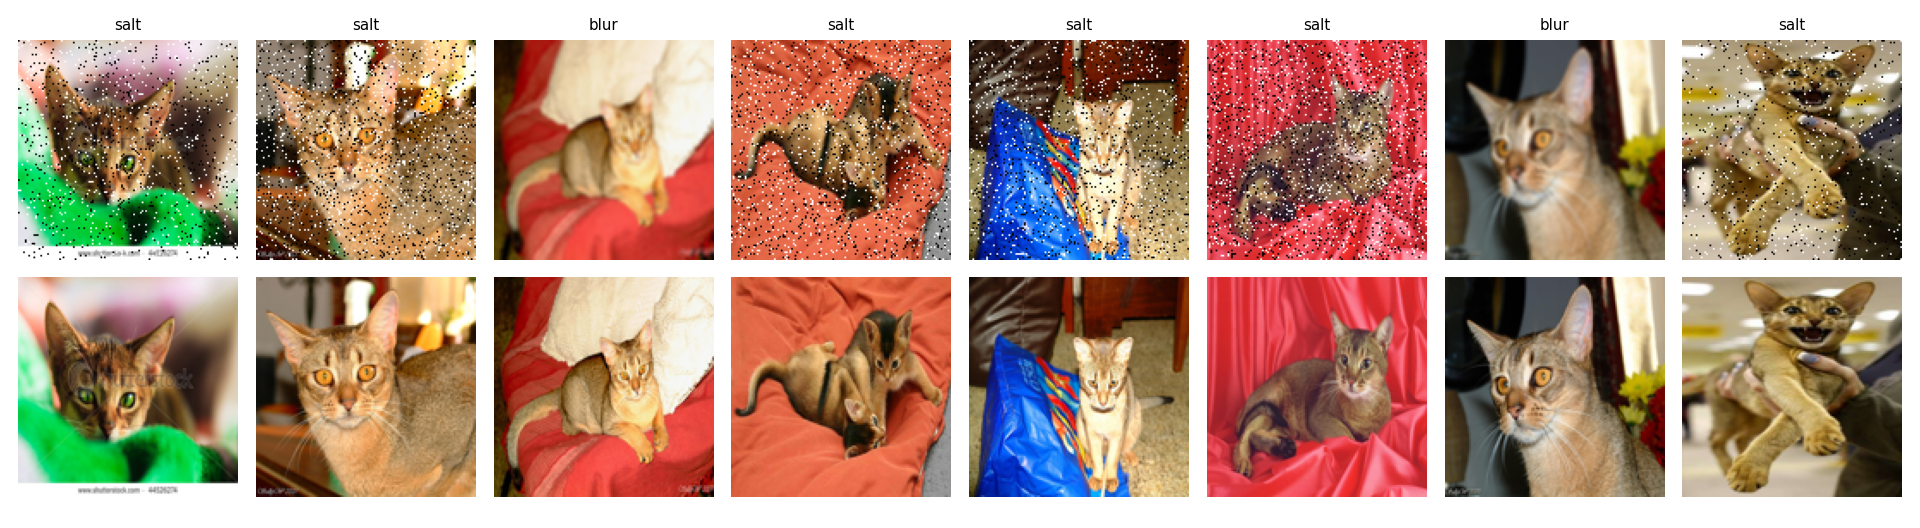
\includegraphics[width=\columnwidth]{data_train_dynamic.png}
\caption{Training-time corruption sampling. Each mini-batch draws a fresh corruption type and fresh parameters from the ranges in Table~\ref{tab:corrupt}, so the model sees a continuous degradation distribution rather than nine discrete settings. This is what prevents the autoencoder from memorising the test grid.}
\label{fig:traindyn}
\end{figure}

\begin{figure}[t]
\centering
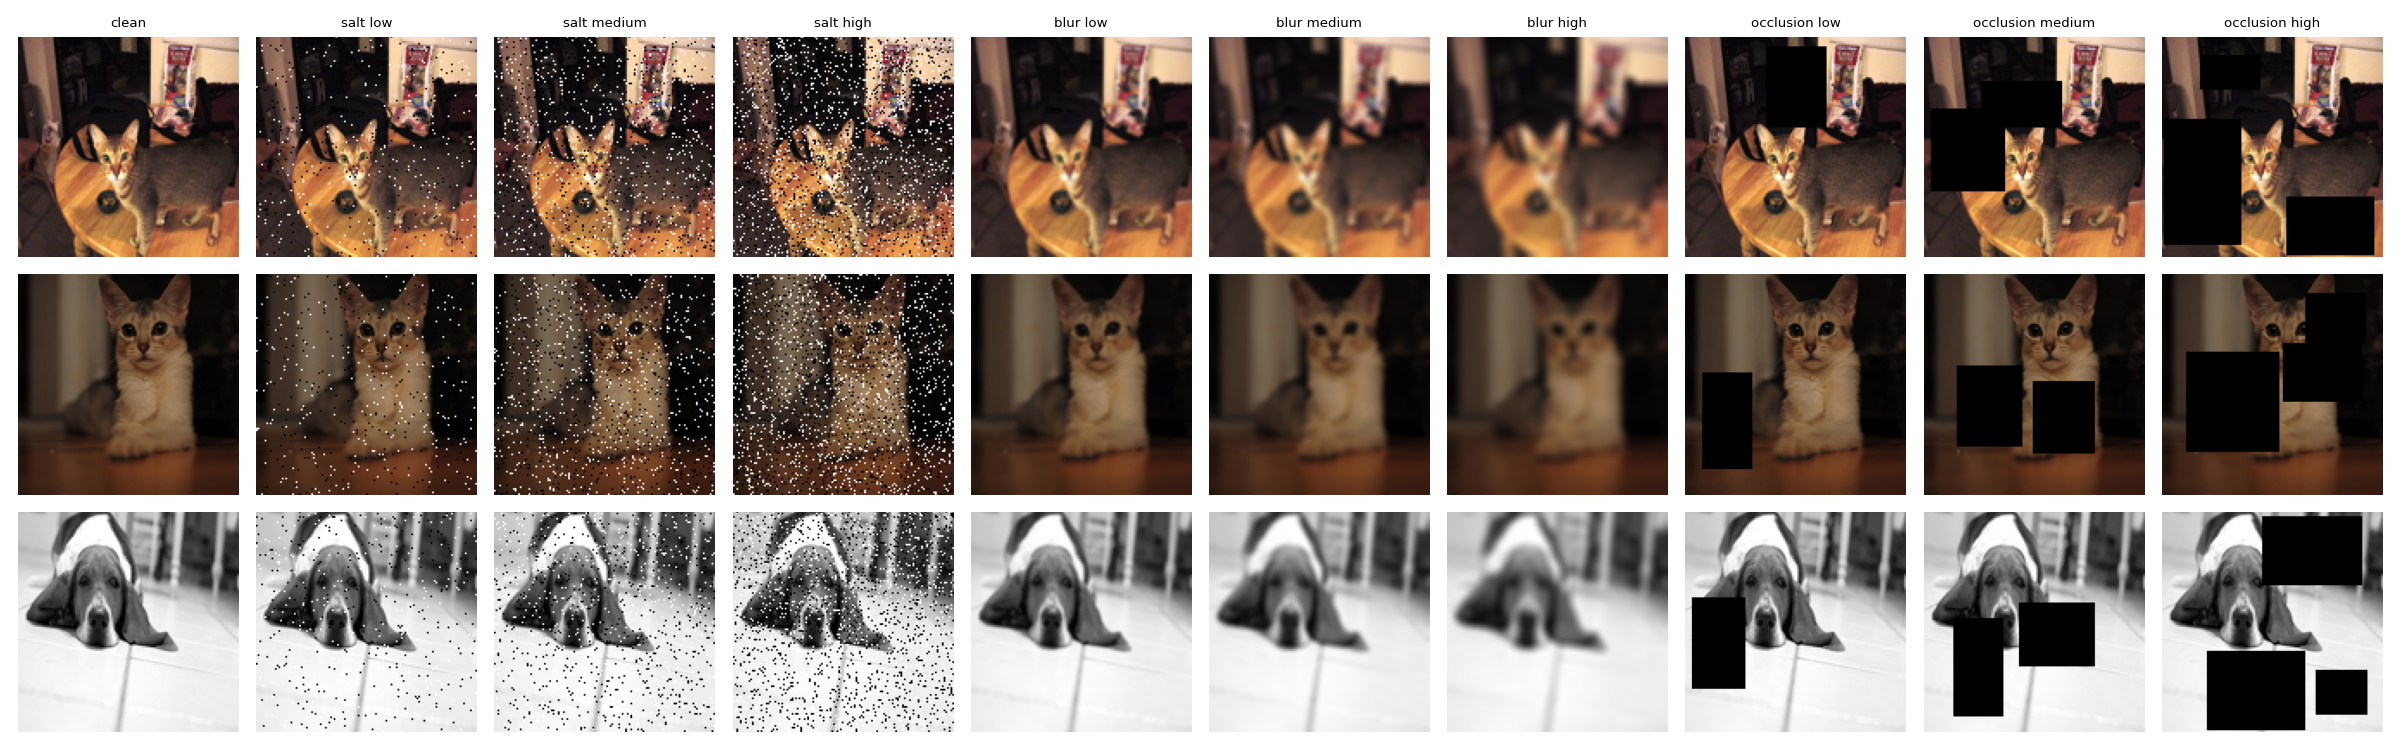
\includegraphics[width=\columnwidth]{data_test_severities.png}
\caption{The nine fixed test conditions --- three corruptions at three severities --- plus the clean control. Evaluation in \S\ref{sec:results} reports every cell of this grid separately rather than a single pooled average, because pooling would hide the severity dependence analysed in Fig.~\ref{fig:t1curves}(b).}
\label{fig:testsev}
\end{figure}

Figure~\ref{fig:traindyn} illustrates the training-time sampler: parameters are redrawn per image, giving a continuum of degradations. Figure~\ref{fig:testsev} shows the discrete evaluation grid that every results table in this paper mirrors cell-for-cell. The contrast between the two figures is the reason training uses ranges while testing uses fixed points.

% ===========================================================================
\section{Architecture Design}
\label{sec:arch}
% ===========================================================================

All four models share one interface contract --- $128\times128$ RGB in, $128\times128$ out (or a style-conditioned sketch) --- so that a single HTTP layer, a single metrics module, and a single ONNX registry can host all of them. The diagrams in this section use one visual language: cyan for data path, violet for learned routing or conditioning, amber for supervision signals that exist only during training.

\subsection{Task 1: plain convolutional autoencoder}
\label{sec:arch1}

\begin{figure}[t]
\centering
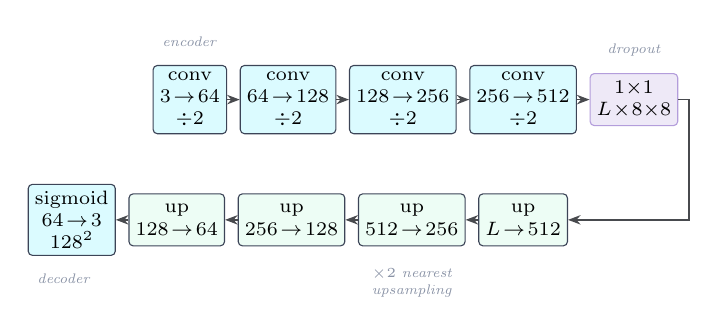
\begin{tikzpicture}[
  font=\scriptsize,
  box/.style={draw=stitchgrid, rounded corners=1.5pt, align=center, inner sep=2.4pt, minimum height=6.6mm},
  enc/.style={box, fill=stitchcyan!14},
  dec/.style={box, fill=stitchgreen!12},
  lat/.style={box, fill=stitchviolet!22, draw=stitchviolet},
  arr/.style={-{Stealth[length=1.6mm]}, semithick, draw=stitchink!75},
  lbl/.style={font=\tiny\itshape, text=stitchmute, align=center}
]
\node[enc, minimum width=9mm] (e1) {conv\\$3\!\to\!64$\\$\div 2$};
\node[enc, minimum width=9mm, right=1.6mm of e1] (e2) {conv\\$64\!\to\!128$\\$\div 2$};
\node[enc, minimum width=9mm, right=1.6mm of e2] (e3) {conv\\$128\!\to\!256$\\$\div 2$};
\node[enc, minimum width=9mm, right=1.6mm of e3] (e4) {conv\\$256\!\to\!512$\\$\div 2$};
\node[lat, minimum width=8mm, right=1.6mm of e4] (z) {$1{\times}1$\\$L\!\times\!8{\times}8$};

\node[dec, minimum width=9mm, below=7.5mm of e4] (d4) {up\\$L\!\to\!512$};
\node[dec, minimum width=9mm, left=1.6mm of d4] (d3) {up\\$512\!\to\!256$};
\node[dec, minimum width=9mm, left=1.6mm of d3] (d2) {up\\$256\!\to\!128$};
\node[dec, minimum width=9mm, left=1.6mm of d2] (d1) {up\\$128\!\to\!64$};
\node[box, fill=stitchcyan!14, left=1.6mm of d1] (out) {sigmoid\\$64\!\to\!3$\\$128^2$};

\draw[arr] (e1) -- (e2); \draw[arr] (e2) -- (e3); \draw[arr] (e3) -- (e4); \draw[arr] (e4) -- (z);
\draw[arr] (z.east) -- ++(1.4mm,0) |- (d4.east);
\draw[arr] (d4) -- (d3); \draw[arr] (d3) -- (d2); \draw[arr] (d2) -- (d1); \draw[arr] (d1) -- (out);

\node[lbl, above=1.1mm of e1.north west, anchor=south west] {encoder};
\node[lbl, below=1.1mm of out.south west, anchor=north west] {decoder};
\node[lbl, above=0.9mm of z.north] {dropout};
\node[lbl, below=1.6mm of d3.south] {$\times 2$ nearest\\upsampling};
\end{tikzpicture}
\caption{\taskname{Task 1} --- plain convolutional autoencoder with no skip connections. Four stride-2 stages compress $128\times128\times3$ to a $L\times8\times8$ latent; four nearest-neighbour upsampling stages restore resolution. Dropout2d is applied at the latent and on the two lowest-resolution decoder stages. The absence of lateral connections is the design constraint that makes the restoration numbers in Table~\ref{tab:t1} meaningful.}
\label{fig:arch1}
\end{figure}

Figure~\ref{fig:arch1} shows the architecture. Each encoder stage is two $3\times3$ conv--BN--ReLU blocks, the first with stride 2, giving four halvings from 128 to 8; a final $1\times1$ convolution projects to $L$ latent channels. The decoder mirrors this with nearest-neighbour upsampling followed by a conv block, and a sigmoid output in $[0,1]$ matching the normalised target. Alternatives considered and rejected: a ResNet-style backbone with skip connections (rejected --- would permit identity shortcuts); tanh output with $[-1,1]$ normalisation (rejected --- $L_1$ and SSIM are computed in $[0,1]$ throughout Tasks~1--3, and consistency across the suite was worth more than the marginal gradient benefit); and a larger $16\times16$ latent with two fewer stages (rejected --- the $8\times8$ bottleneck is what forces semantic rather than pixel-level encoding, and Optuna's search space in Table~\ref{tab:optuna} confirmed that larger latent \emph{channel} counts win while spatial resolution stayed fixed).

\subsection{Task 2: classifier-gated hard routing}
\label{sec:arch2}

\begin{figure}[t]
\centering
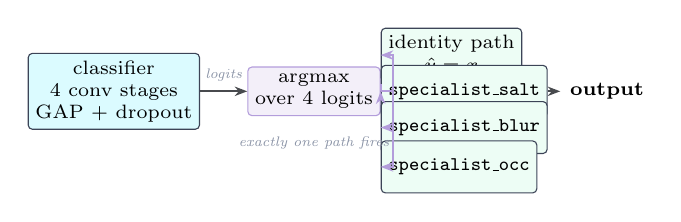
\begin{tikzpicture}[
  font=\scriptsize,
  box/.style={draw=stitchgrid, rounded corners=1.5pt, align=center, inner sep=2.6pt, minimum height=6.6mm},
  cls/.style={box, fill=stitchcyan!14},
  sw/.style={draw=stitchviolet, fill=stitchviolet!16, rounded corners=1.5pt, align=center, inner sep=2.6pt},
  exp/.style={box, fill=stitchgreen!12},
  arr/.style={-{Stealth[length=1.6mm]}, semithick, draw=stitchink!75},
  varr/.style={-{Stealth[length=1.6mm]}, semithick, draw=stitchviolet},
  lbl/.style={font=\tiny\itshape, text=stitchmute, align=center}
]
\node[cls, minimum width=15mm] (c) {classifier\\4 conv stages\\GAP + dropout};
\node[sw, minimum width=13mm, right=6mm of c] (sw) {argmax\\over 4 logits};
\node[exp, minimum width=17mm, above=4.6mm of sw.east, anchor=west] (e0) {identity path\\$\hat y = x$};
\node[exp, minimum width=17mm, right=0mm of sw.east] (e1) {\texttt{specialist\_salt}};
\node[exp, minimum width=17mm, below=4.6mm of sw.east, anchor=west] (e2) {\texttt{specialist\_blur}};
\node[exp, minimum width=17mm, below=9.6mm of sw.east, anchor=west] (e3) {\texttt{specialist\_occ}};
\node[right=1.6mm of e1.east] (o) {\textbf{output}};

\draw[arr] (c) -- node[lbl, above]{logits} (sw);
\draw[varr] (sw.east) -- ++(1.6mm,0) |- (e0.west);
\draw[varr] (sw.east) -- (e1.west);
\draw[varr] (sw.east) -- ++(1.6mm,0) |- (e2.west);
\draw[varr] (sw.east) -- ++(1.6mm,0) |- (e3.west);
\draw[arr] (e1.east) -- (o);
\node[lbl, below=1.4mm of sw.south] {exactly one path fires};
\end{tikzpicture}
\caption{\taskname{Task 2} --- hard routing. A four-way classifier produces logits; the argmax selects exactly one of four paths. The identity path is a genuine class (an uncorrupted input should be passed through untouched), and the three specialists are Task-1-style autoencoders trained individually on one corruption each. Only the selected specialist's parameters receive gradient for a given image, so each specialises without interference.}
\label{fig:arch2}
\end{figure}

Figure~\ref{fig:arch2} shows hard routing. The classifier and each specialist are trained separately --- classifier on the classification objective, specialists on the restoration objective restricted to their own corruption --- and only at inference are they composed. This decoupling is the key architectural decision: it means a failure can be attributed unambiguously to either identification or restoration, which is exactly the distinction the confusion matrix in Fig.~\ref{fig:t2cm} and the per-corruption rows of Table~\ref{tab:t2} make possible. A single end-to-end routed network with a straight-through argmax was considered and rejected: at this scale the added training complexity buys nothing measurable, and it destroys the interpretability that motivates hard routing in the first place.

\subsection{Task 3: soft mixture-of-experts}
\label{sec:arch3}

\begin{figure}[t]
\centering
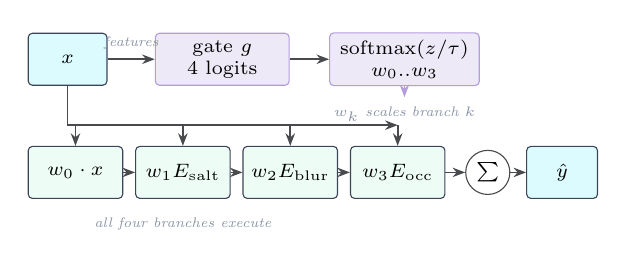
\begin{tikzpicture}[
  font=\scriptsize,
  box/.style={draw=stitchgrid, rounded corners=1.5pt, align=center, inner sep=2.4pt, minimum height=6.6mm},
  gate/.style={box, fill=stitchviolet!22, draw=stitchviolet},
  exp/.style={box, fill=stitchgreen!12},
  sum/.style={draw=stitchink!75, circle, inner sep=1.4pt, minimum size=5.6mm},
  arr/.style={-{Stealth[length=1.6mm]}, semithick, draw=stitchink!75},
  varr/.style={-{Stealth[length=1.6mm]}, semithick, draw=stitchviolet},
  lbl/.style={font=\tiny\itshape, text=stitchmute, align=center}
]
\node[box, fill=stitchcyan!14, minimum width=10mm] (x) {$x$};
\node[gate, minimum width=17mm, right=6mm of x] (g) {gate $g$\\4 logits};
\node[gate, minimum width=19mm, right=5mm of g] (sm) {$\mathrm{softmax}(z/\tau)$\\$w_0..w_3$};

\node[lbl, below=1.4mm of sm.south] {$w_k$ scales branch $k$};
\draw[varr] (sm.south) -- ($(sm.south)+(0,-1.4mm)$);

\node[exp, minimum width=12mm, below=11mm of x.south west, anchor=west] (b0) {$w_0\cdot x$};
\node[exp, minimum width=12mm, right=1.5mm of b0] (b1) {$w_1 E_{\text{salt}}$};
\node[exp, minimum width=12mm, right=1.5mm of b1] (b2) {$w_2 E_{\text{blur}}$};
\node[exp, minimum width=12mm, right=1.5mm of b2] (b3) {$w_3 E_{\text{occ}}$};
\node[sum, right=2.5mm of b3] (s) {$\sum$};
\node[box, fill=stitchcyan!14, right=2mm of s, minimum width=9mm] (o) {$\hat y$};

% input fan-out: one bus above the branch row, one arrow into each branch
\draw[arr] (x.south) -- ++(0,-5mm) coordinate (bus) -- (b3.north |- bus);
\foreach \b in {b0,b1,b2,b3} \draw[arr] (\b.north |- bus) -- (\b.north);

\draw[arr] (x) -- node[lbl, above]{features} (g);
\draw[arr] (g) -- (sm);
\draw[arr] (b0) -- (b1); \draw[arr] (b1) -- (b2); \draw[arr] (b2) -- (b3);
\draw[arr] (b3) -- (s);
\draw[arr] (s) -- (o);
\node[lbl, below=1.2mm of b1.south] {all four branches execute};
\end{tikzpicture}
\caption{\taskname{Task 3} --- soft mixture-of-experts. The same gate produces four logits, but a temperature-scaled softmax converts them into convex weights $w_k$ that sum to one. Unlike Fig.~\ref{fig:arch2}, every path executes on every image and the outputs are blended, so ambiguous inputs are shared across specialists instead of forced onto one. The identity branch $w_0\cdot x$ gives the gate a no-op option; $\tau$ controls sharpness and was itself searched by Optuna.}
\label{fig:arch3}
\end{figure}

Figure~\ref{fig:arch3} shows the soft model. Formally the output is
\begin{equation}
\hat y \;=\; \sum_{k=0}^{3} w_k \, f_k(x),
\qquad
w \;=\; \mathrm{softmax}\!\big(g(x)/\tau\big),
\label{eq:moe}
\end{equation}
where $f_0(x)=x$ is the identity branch and $f_1,f_2,f_3$ are the salt, blur, and occlusion specialists. Three design points deserve justification. \emph{The identity branch is a branch, not an expert}: it has no parameters, so the gate cannot learn to route clean images through a network that would only perturb them. \emph{Temperature $\tau$ matters}: at $\tau\!\to\!0$ Eq.~\eqref{eq:moe} collapses to Task 2's hard routing, and at $\tau\!\to\!\infty$ it degenerates to a uniform average of all specialists, which would destroy specialisation; searching $\tau$ over $[0.5,2.0]$ lets Optuna place it where the data wants it. \emph{All four paths execute}: unlike sparse MoE, there is no compute saving here --- the gain being sought is accuracy on ambiguous and compound inputs, not FLOPs, which is why no load-balancing term beyond the mild one in \S\ref{sec:loss} is needed.

\subsection{Task 4: style-conditioned sketch GAN}
\label{sec:arch4}

\begin{figure}[t]
\centering
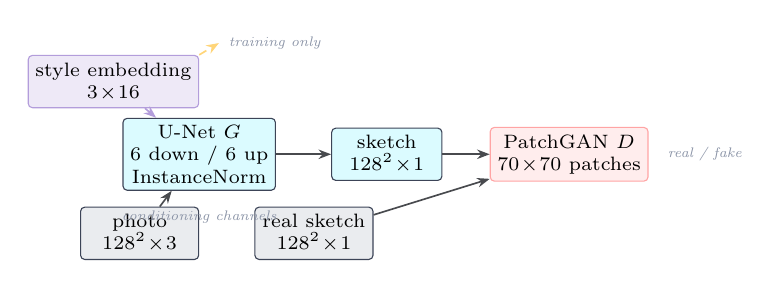
\begin{tikzpicture}[
  font=\scriptsize,
  box/.style={draw=stitchgrid, rounded corners=1.5pt, align=center, inner sep=2.6pt, minimum height=6.6mm},
  gen/.style={box, fill=stitchcyan!14},
  dis/.style={box, fill=stitchcoral!14, draw=stitchcoral!70},
  emb/.style={box, fill=stitchviolet!22, draw=stitchviolet},
  arr/.style={-{Stealth[length=1.6mm]}, semithick, draw=stitchink!75},
  varr/.style={-{Stealth[length=1.6mm]}, semithick, draw=stitchviolet},
  amar/.style={-{Stealth[length=1.6mm]}, semithick, draw=stitchamber!80},
  lbl/.style={font=\tiny\itshape, text=stitchmute, align=center}
]
\node[gen, minimum width=15mm] (g) {U-Net $G$\\6 down / 6 up\\InstanceNorm};
\node[emb, minimum width=13mm, above=4.6mm of g.north, anchor=east] (s) {style embedding\\$3\!\times\!16$};
\node[gen, minimum width=14mm, right=7mm of g] (sk) {sketch\\$128^2\!\times\!1$};
\node[dis, minimum width=17mm, right=6mm of sk] (d) {PatchGAN $D$\\$70\!\times\!70$ patches};
\node[lbl, right=1.2mm of d.east] (rf) {real / fake};

\node[box, fill=stitchmute!18, minimum width=15mm, below=5.4mm of g.south, anchor=east] (ph) {photo\\$128^2\!\times\!3$};
\node[box, fill=stitchmute!18, minimum width=15mm, right=7mm of ph] (gt) {real sketch\\$128^2\!\times\!1$};

\draw[arr] (ph) -- (g);
\draw[varr] (s) -- (g);
\draw[arr] (g) -- (sk);
\draw[arr] (sk) -- (d);
\draw[arr] (gt) -- (d);
\draw[amar, dashed] (s.north east) -- ++(2.5mm,1.5mm) node[lbl, right]{training only};
\node[lbl, below=1.3mm of g.south] {conditioning channels};
\end{tikzpicture}
\caption{\taskname{Task 4} --- conditional sketch GAN. The photo enters the U-Net generator; a learned style embedding is broadcast and concatenated to the input channels, adding 16 conditioning channels to the 3 RGB channels so one generator serves all three FS2K styles. A PatchGAN discriminator judges $70\times70$ patches of (generated or real) sketch. Dashed amber path exists only during training.}
\label{fig:arch4}
\end{figure}

Figure~\ref{fig:arch4} shows the generator and discriminator. The generator is a U-Net: six stride-2 downsampling blocks with InstanceNorm and LeakyReLU ($\alpha=0.2$), a bottleneck, and six transposed-convolution blocks with InstanceNorm and ReLU, with a `tanh' output in $[-1,1]$. Skip connections are retained here \emph{deliberately}, in contrast to Task~1: photo-to-sketch translation must preserve spatial layout, so high-frequency geometry has to travel from encoder to decoder; the adversarial objective, not a restoration bottleneck, is responsible for the stylistic transform. Conditioning is implemented by concatenating a $16$-dimensional style embedding, learned by \texttt{nn.Embedding}, broadcast across the spatial dimensions and appended to the input channels --- a simpler and more stable alternative to FiLM-style affine modulation, which was considered but rejected because with only three styles and 899 training pairs the extra parameters had no data to fit. Dropout in the decoder provides the stochasticity that lets a single generator produce variation across styles rather than a deterministic collapse to the majority style.

% ===========================================================================
\section{Loss Functions}
\label{sec:loss}
% ===========================================================================

\subsection{Restoration (Tasks 1--3)}

Tasks~1 and~2 minimise
\begin{equation}
\mathcal{L}_{\text{rest}} \;=\; \alpha \, \lVert \hat y - y \rVert_1 \;+\; (1-\alpha)\,\big(1-\mathrm{SSIM}(\hat y, y)\big),
\label{eq:rest}
\end{equation}
with $\alpha$ searched rather than fixed. $L_1$ anchors pixel accuracy; the SSIM term pushes the model toward structurally plausible output, which a pure $L_1$ objective under-weighted in preliminary runs (it converges to a conditional mean that is perceptually over-smooth). Setting $\alpha=0.5$, the best Task-1 value, balances them; Task 3's $\alpha=0.55$ tilts marginally toward $L_1$.

Task 3 adds two routing terms to Eq.~\eqref{eq:rest}:
\begin{equation}
\mathcal{L}_3 \;=\; \mathcal{L}_{\text{rest}} \;+\; \lambda_c\,\mathcal{L}_{\text{CE}}\!\big(g(x),\, t\big) \;+\; \lambda_b\,\mathcal{L}_{\text{bal}}(w),
\label{eq:task3}
\end{equation}
where $\mathcal{L}_{\text{CE}}$ is cross-entropy against the known corruption label $t$ and $\mathcal{L}_{\text{bal}}$ is a routing-balance term discouraging the gate from collapsing onto one branch. Both weights were searched over wide log ranges ($\lambda_c\in[0.01,1]$, $\lambda_b\in[10^{-3},1]$) and both came out \emph{small} --- $\lambda_c=0.017$, $\lambda_b=0.0022$ in the best trial --- which is itself a result: the reconstruction signal was sufficient to induce specialisation, and the auxiliary terms were only needed to prevent degenerate collapse. The balance weight landing two orders of magnitude below its ceiling indicates the balance term is a safety net rather than a load-bearing objective.

\subsection{Classification (Task 2)}

The classifier minimises standard multi-class cross-entropy with label smoothing off and weight decay searched over $[10^{-6},10^{-2}]$. Class balance is handled in the \emph{sampler}, not the loss: batches are drawn with $\lfloor B/4\rfloor$ examples per class, which is preferable to inverse-frequency loss weighting here because it gives every update a clean four-class gradient rather than up-weighting rare examples into high-variance updates.

\subsection{Adversarial translation (Task 4)}

The generator objective combines a least-squares adversarial term with a heavily weighted $L_1$ term,
\begin{equation}
\mathcal{L}_G = \mathcal{L}_{\text{adv}}^{(\text{ls})}\big(D(G(x,s)),\,1\big)
  + \lambda_{L1}\,\lVert G(x,s) - y \rVert_1 ,
\end{equation}
and the discriminator distinguishes real from generated patches with $\mathcal{L}_D=\tfrac12\big[\mathcal{L}^{(\text{ls})}(D(y),1)+\mathcal{L}^{(\text{ls})}(D(G(x,s)),0)\big]$. $\lambda_{L1}=200$ was fixed rather than searched after a short pilot showed the generator ignoring content alignment below 50 and becoming unstable above 400; the searched variables were $\mathrm{lr}_G$, $\mathrm{lr}_D$, batch size, width, dropout, and embedding dimension. The least-squares formulation was chosen over the logistic loss because it supplies non-saturating gradients when the discriminator is already confident, which was observed to be the failure mode in early Task-4 runs.

% ===========================================================================
\section{Training Procedure}
\label{sec:train}
% ===========================================================================

\begin{figure*}[t]
\centering
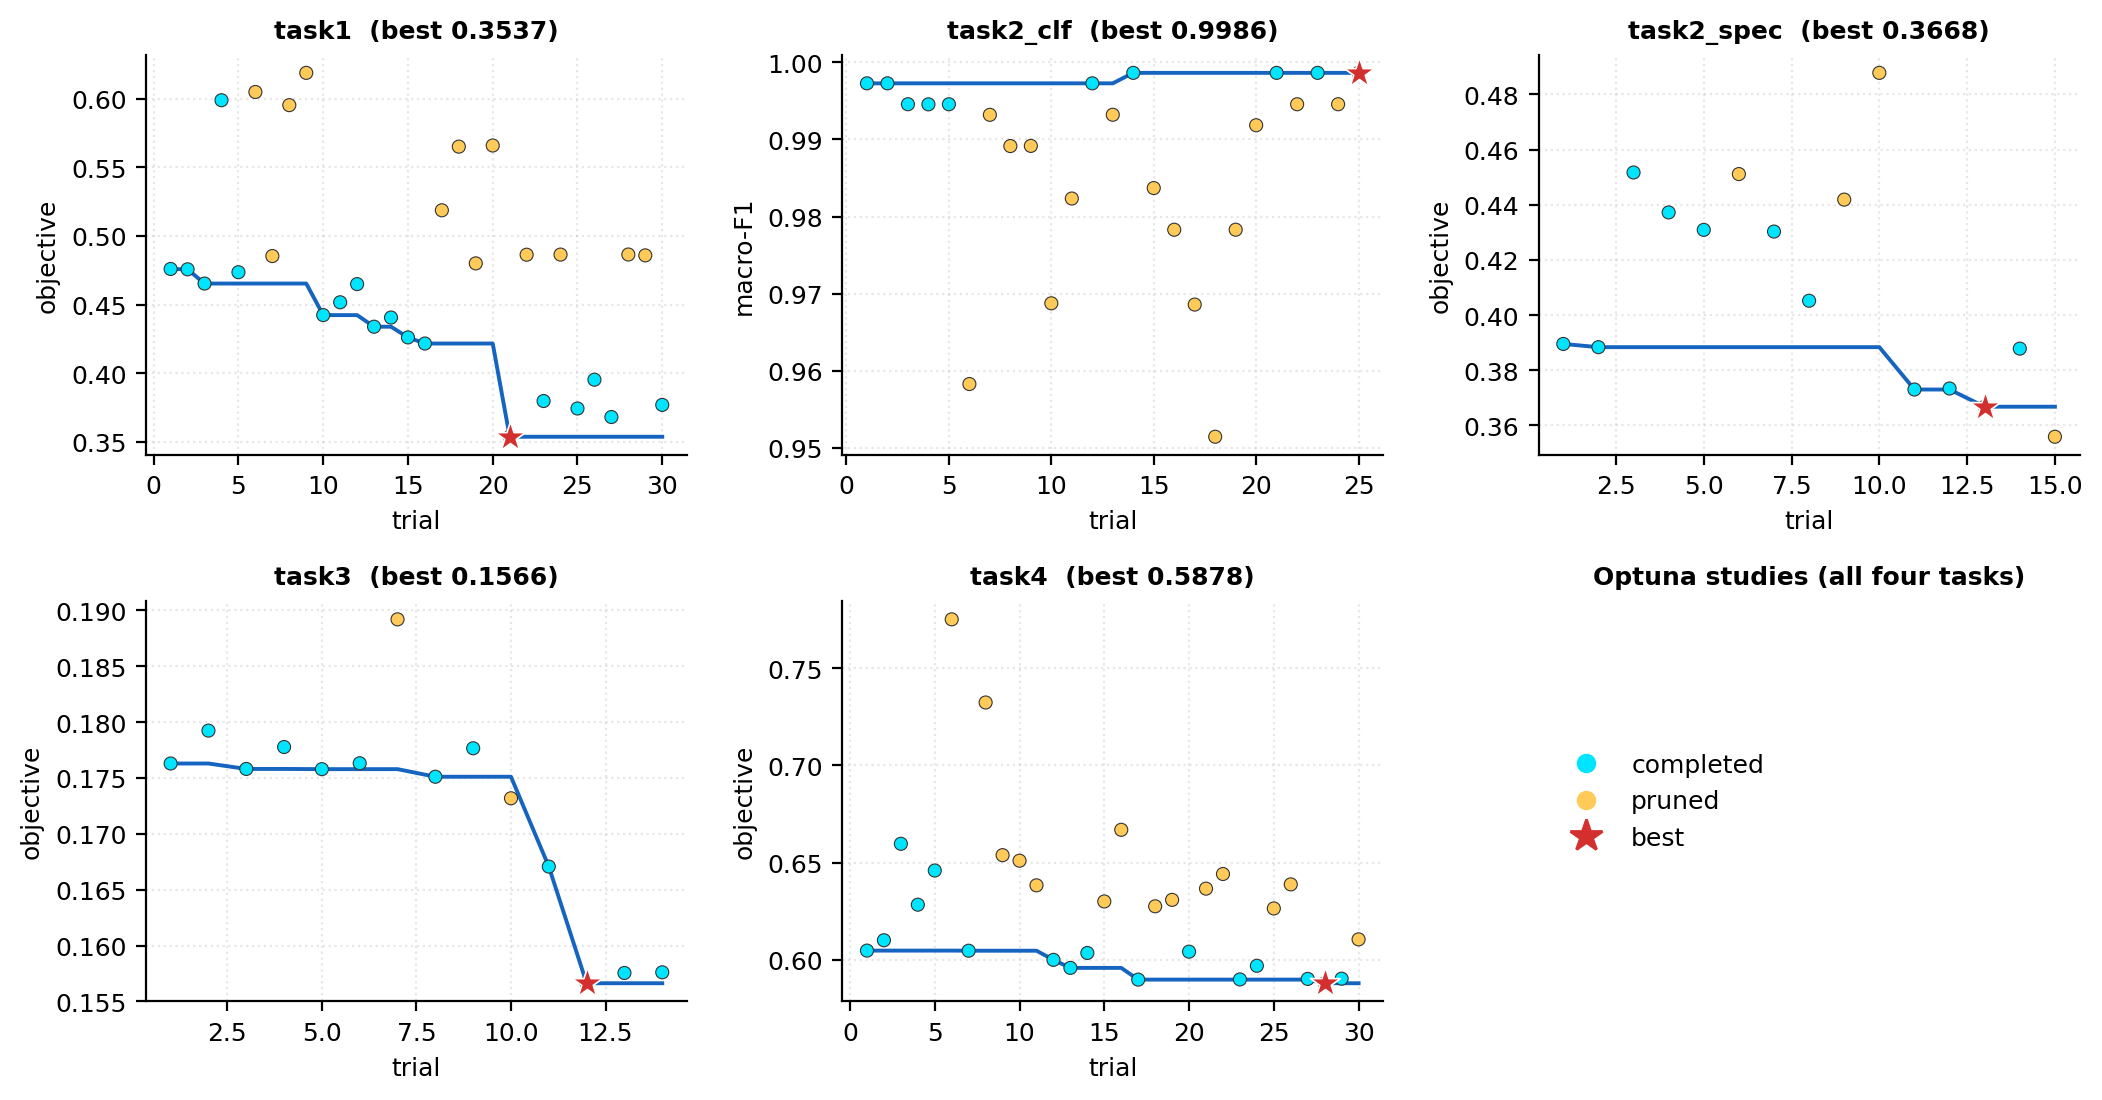
\includegraphics[width=0.98\textwidth]{optuna_studies.png}
\caption{Optuna search trajectories for all five studies. Each point is a trial; cyan marks completed, amber pruned, grey failed; the blue line is the running best over completed trials only and the red star the selected trial. Objective is minimised for Tasks 1, 2-specialist, 3, and 4, and \emph{maximised} (macro-F1) for the Task-2 classifier. Pruning eliminated 12/30, 15/25, 4/17, 2/14, and 14/30 trials respectively, so the reported bests come from 18, 10, 11, 12, and 16 fully trained configurations. Note the Task-2 classifier study converges almost immediately --- its objective saturates near 0.999 within a handful of trials --- while Task 1 and Task 4 show the long, gradual improvement characteristic of reconstruction objectives.}
\label{fig:optuna}
\end{figure*}

\subsection{Optimisation and schedules}

All restoration models use Adam~\cite{kingma2015adam} with default moment parameters. Task 1 trains for 100 epochs with the selected learning rate and batch size, selecting the checkpoint by validation objective rather than by final epoch (the reported test numbers come from epoch 97, not 100 --- see Fig.~\ref{fig:t1curves}(a), where validation loss has flattened but not yet begun to drift upward). The classifier trains for 60 epochs.

Task 3 uses a \emph{two-stage} schedule, which is the one genuinely novel training procedure in the suite. Stage 1 warms up the gate alone for 2 epochs at a fixed $3\times10^{-4}$ while the pretrained Task-2 specialists are frozen; stage 2 fine-tunes gate and experts jointly for the remaining epochs at the searched $\mathrm{lr}_{ft}$. The rationale is that an randomly initialised gate supervising unfrozen experts produces meaningless gradients into the experts for the first epochs, and experts that begin drifting before the gate is even weakly calibrated are hard to recover. Fig.~\ref{fig:t3curves}(a) shades the warm-up window and shows joint loss falling steeply once unfrozen --- evidence that the schedule is doing work rather than merely delaying. The searched $\mathrm{lr}_{ft}=3.06\times10^{-5}$ is notably smaller than the warm-up rate, consistent with fine-tuning a co-trained system rather than training from scratch.

Task 4 trains for 150 epochs with separate generator and discriminator learning rates, checkpointing on validation objective (best epoch 93 of 150 --- the generator does not simply improve monotonically, which Fig.~\ref{fig:t4curves}(b) shows directly).

\subsection{Checkpointing, tracking, and reproducibility}

Every run logs to MLflow: per-epoch train and validation metrics, the selected configuration, and sample image grids. Random seeds are set for NumPy, PyTorch, and Python's \texttt{random}; occlusion generation additionally carries an explicit per-image seed so a test corruption is bit-reproducible across a re-run and across the HTTP API. Test metrics are written as JSON and CSV artifacts that the deployed backend reads directly, which is what populates the ``recorded test results'' panel visible in the application screenshots in Figs.~\ref{fig:app1}--\ref{fig:app4}: the browser shows the same numbers reported here, not a re-computation.

% ===========================================================================
\section{Hyperparameter Search with Optuna}
\label{sec:optuna}
% ===========================================================================

Table~\ref{tab:optuna} lists the five studies. All use Optuna's TPE sampler with a median pruner: a trial whose intermediate validation objective is below the median of completed trials at the same step is stopped early. This is why Fig.~\ref{fig:optuna} contains so many amber points --- pruning is doing most of the work in making the search affordable.

\begin{table*}[t]
\caption{Optuna study summary. ``Best'' is over completed trials only; a pruned trial can transiently hold a better intermediate value, so including pruned trials would report a number no trained model actually achieves. Task 2 is split into two studies: the classifier (maximising macro-F1) and the three specialists jointly (minimising mean restoration objective).}
\label{tab:optuna}
\centering
\scriptsize
\setlength{\tabcolsep}{5pt}
\begin{tabular}{@{}lccccp{6.1cm}@{}}
\toprule
\textbf{Study} & \textbf{Trials} & \textbf{Done} & \textbf{Pruned} & \textbf{Best} & \textbf{Objective}\\
\midrule
Task 1 --- autoencoder      & 30 & 18 & 12 & 0.3537 & $\mathrm{val\_l1} + (1-\mathrm{val\_ssim})$\\
Task 2 --- classifier       & 25 & 10 & 15 & 0.9986 & validation macro-F1 (maximise)\\
Task 2 --- specialists      & 17 & 11 & 4  & 0.3668 & mean over 3 specialists of $\mathrm{val\_l1}+1-\mathrm{val\_ssim}$\\
Task 3 --- soft MoE         & 14 & 12 & 2  & 0.1566 & $\mathrm{val\_l1}+(1-\mathrm{val\_ssim})$ at best post-warm-up epoch\\
Task 4 --- sketch GAN       & 30 & 16 & 14 & 0.5878 & validation objective at best epoch\\
\bottomrule
\end{tabular}
\end{table*}

\begin{table}[t]
\caption{Selected hyperparameters per study (post-search). Categorical values are shown verbatim; note that every study independently selected either the widest channel configuration or a large latent, suggesting under-capacity rather than over-capacity was the binding constraint at this scale.}
\label{tab:best}
\centering
\scriptsize
\setlength{\tabcolsep}{3.2pt}
\begin{tabular}{@{}lp{6.0cm}@{}}
\toprule
\textbf{Study} & \textbf{Best hyperparameters}\\
\midrule
Task 1 & $\mathrm{lr}=1.06{\times}10^{-3}$, $B=16$, \texttt{latent}=64, \texttt{base}=64, \texttt{drop}=0.0, $\alpha=0.5$\\
Task 2 clf & $\mathrm{lr}=1.50{\times}10^{-4}$, $B=32$, \texttt{wide}=[48,96,192,256], \texttt{drop}=0.5, $\mathrm{wd}=1.13{\times}10^{-4}$\\
Task 2 spec & $\mathrm{lr}$, $B$, width and regularisation tuned per specialist (Table~\ref{tab:optuna})\\
Task 3 & $\mathrm{lr}_{ft}=3.06{\times}10^{-5}$, $\tau=1.526$, $\lambda_c=0.0174$, $\lambda_b=0.0022$, $\alpha=0.55$, $B=32$\\
Task 4 & $\mathrm{lr}_G=7.56{\times}10^{-4}$, $\mathrm{lr}_D=1.07{\times}10^{-4}$, $B=4$, \texttt{base}=48, \texttt{drop}=0.3, \texttt{emb}=16, $\lambda_{L1}=200$\\
\bottomrule
\end{tabular}
\end{table}

Figure~\ref{fig:optuna} plots all five studies together, and Table~\ref{tab:best} gives the winning configurations. Four observations follow from reading them side by side.

\emph{Pruning rates differ by an order of magnitude across tasks.} The classifier pruned 15 of 25 trials (60\%) while Task 3 pruned only 2 of 14 (14\%). The classifier's objective can be estimated reliably from a few epochs, so early stopping is safe; Task 3's objective depends on a two-stage warm-up schedule whose outcome is only legible after both stages run, so there is little to prune. Pruning budget should therefore be task-specific rather than set globally.

\emph{The classifier study saturates almost immediately.} Its running-best line in Fig.~\ref{fig:optuna} is essentially flat after trial 5, meaning the search space was too easy relative to the problem --- accuracy was already near ceiling. The remaining trials bought robustness (dropout 0.5, weight decay $10^{-4}$) rather than accuracy.

\emph{Capacity was never the bottleneck.} Every study that searched width selected the largest option: Task 1 chose \texttt{latent}=64 and \texttt{base}=64 (the top of both ranges), and Task 2 chose the \texttt{wide} channel schedule. With $128\times128$ inputs and 899--1058 training images, models were under-, not over-, capacity-limited --- despite dropout and weight decay being available as regularisers.

\emph{Task 4's search was the least conclusive.} Its running-best line improves in visible steps throughout the 30 trials without plateauing, which indicates the search had not converged; combined with the small style-2 test subset identified in \S\ref{sec:results4}, this is the clearest signal that more search budget would change Task-4 results.

% ===========================================================================
\section{Experimental Setup}
\label{sec:setup}
% ===========================================================================

\subsection{Splits and evaluation protocol}

Tasks 1--3 share one corpus and one test split of 36{,}690 images: 4 classes $\times$ 3 severities $\times$ 3{,}058 base photographs, plus the clean control. Because every table in \S\ref{sec:results} is computed over this same split, rows are directly comparable \emph{across} tasks --- Table~\ref{tab:t3}, for example, places soft and hard routing on identical inputs. Task 4 evaluates on the 1{,}046 official FS2K test pairs, untouched during model selection; validation for every task comes from a held-out portion of the respective training split.

\subsection{Metrics}

Three metrics are reported. \textbf{L1} is mean absolute pixel error in $[0,1]$. \textbf{PSNR} is $10\log_{10}(1/\mathrm{MSE})$ in dB; clean inputs are reported as `---' where the backend returns \texttt{null} rather than the 100~dB ceiling, because the input \emph{is} the target and the delta is undefined, not zero. \textbf{SSIM} is computed on luminance with an $11\times11$ Gaussian window. For routing tasks a fourth quantity appears: \textbf{gate/routing accuracy}, the fraction of images assigned to the correct branch.

\subsection{Deployment stack}

Models are exported to ONNX and served by FastAPI through an ONNX Runtime session; the browser client is React with Tailwind; nginx serves the built SPA and reverse-proxies \texttt{/api}; Docker Compose wires the two containers and the model volume together. \S\ref{sec:app} describes the full architecture.

% ===========================================================================
\section{Results and Analysis}
\label{sec:results}
% ===========================================================================

\subsection{Task 1 --- single autoencoder}
\label{sec:results1}

\begin{figure*}[t]
\centering
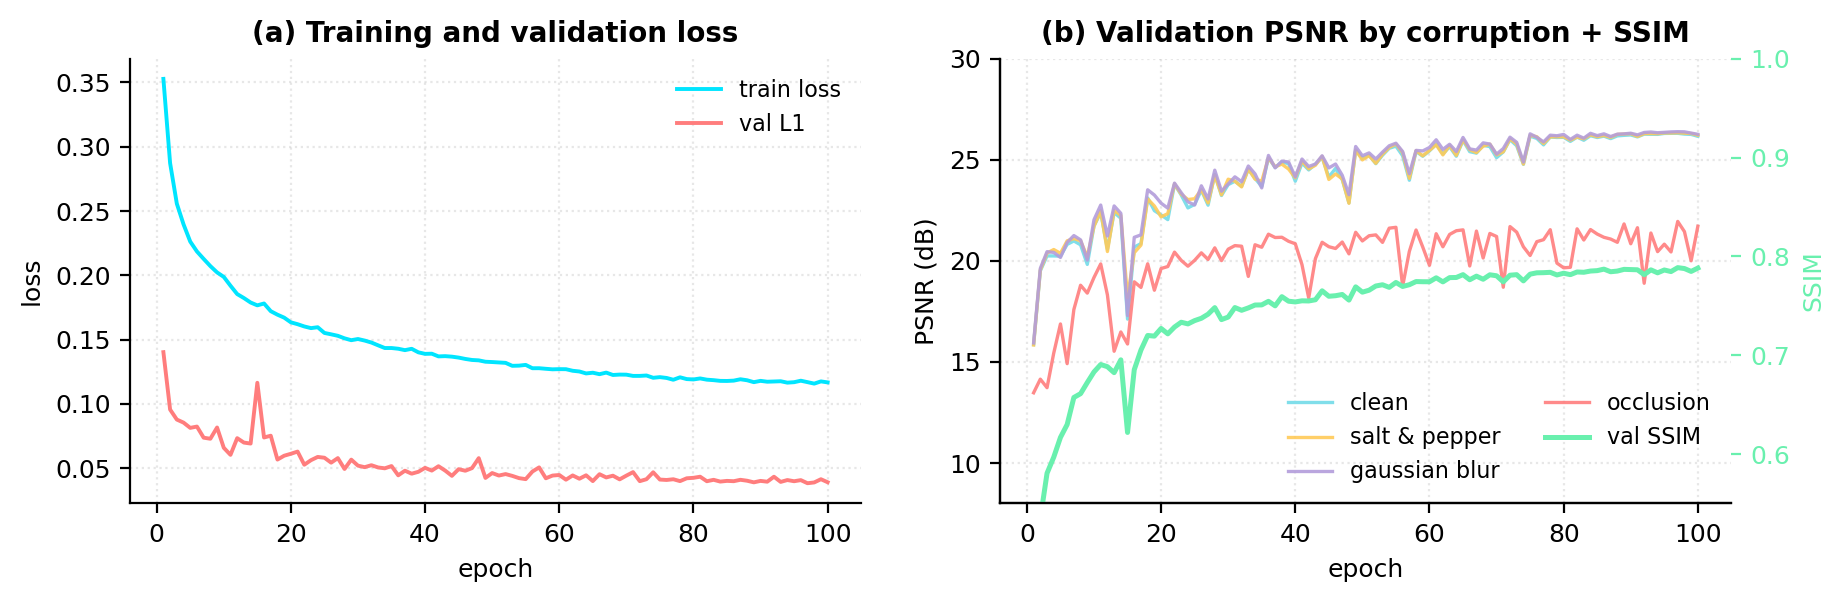
\includegraphics[width=0.9\textwidth]{task1_curves.png}
\caption{\taskname{Task 1} training and validation behaviour over 100 epochs. (a)~Training loss and validation $L_1$ fall together and flatten after epoch $\sim$40, with no train/validation divergence --- the searched dropout of 0.0 was correct for this small, heavily-augmented corpus. (b)~Validation PSNR per corruption on the left axis with overall validation SSIM on the right. The ordering is the paper's central quantitative observation for Task 1: clean inputs sit at $\sim$26~dB, salt at $\sim$26~dB, blur at $\sim$26~dB, but occlusion sits 4--6~dB lower throughout training and never closes the gap. Reconstruction difficulty is determined by the fraction of information destroyed, not by how visible the corruption is --- salt is visually dramatic yet easily inpainted from 85--97\% surviving pixels, while 35\% occlusion removes content that cannot be inferred.}
\label{fig:t1curves}
\end{figure*}

\begin{table}[t]
\caption{\taskname{Task 1} test results by corruption (mean over severities). Input PSNR is the corrupted image against the clean target; output is the restored image. Clean rows are scored for output quality only --- the delta is undefined when the input is the target.}
\label{tab:t1}
\centering
\scriptsize
\setlength{\tabcolsep}{3.6pt}
\begin{tabular}{@{}lrrrr@{}}
\toprule
\textbf{Condition} & \textbf{In PSNR} & \textbf{Out PSNR} & \textbf{$\Delta$ PSNR} & \textbf{Out SSIM}\\
\midrule
clean      & ---  & 26.25 & ---    & 0.814\\
salt       & 16.38 & 26.16 & $+9.77$ & 0.807\\
blur       & 27.82 & 25.91 & $-1.92$ & 0.785\\
occlusion  & 13.57 & 21.98 & $+8.41$ & 0.728\\
\midrule
\textbf{overall} & 27.33 & \textbf{24.84} & --- & \textbf{0.777}\\
\bottomrule
\end{tabular}
\end{table}

\begin{figure*}[t]
\centering
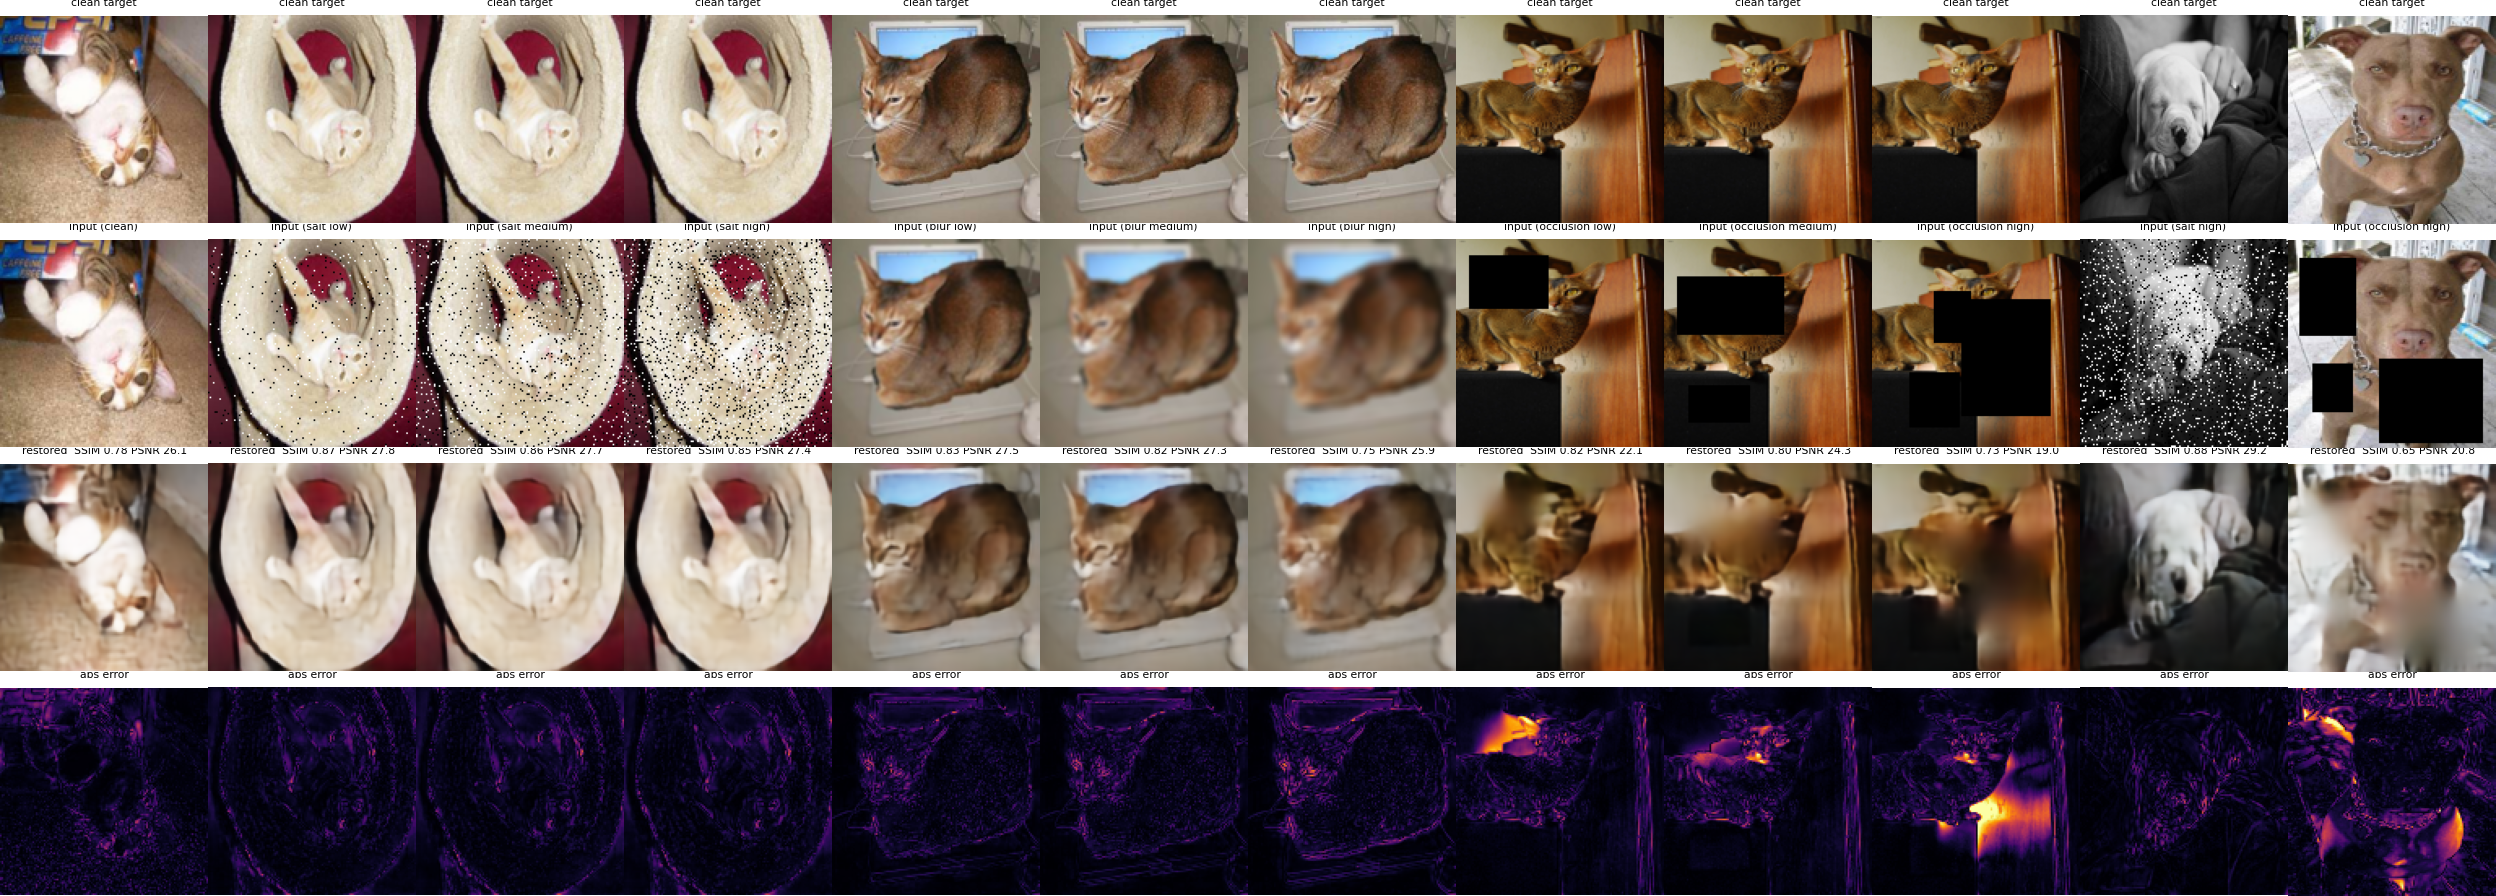
\includegraphics[width=0.98\textwidth]{t1_examples.png}
\caption{\taskname{Task 1} qualitative results. Columns are test conditions (clean, salt at three severities, blur at three, occlusion at three, plus two held-out compound cases); rows are clean target, corrupted input, restored output with its SSIM/PSNR, and absolute error map. Reading down the error column is more informative than reading the restored row: for salt and blur the error maps are dark and spatially uniform, meaning the autoencoder repairs damage evenly across the frame; for occlusion the error maps are bright and \emph{structured}, concentrating on the occluder boundaries where the model must invent content. The two right-most columns, drawn from compound corruptions outside the four-class taxonomy, show the model defaulting to a smooth interpolation --- its correct behaviour given it was never trained on such inputs.}
\label{fig:t1ex}
\end{figure*}

Table~\ref{tab:t1} and Fig.~\ref{fig:t1curves} give Task 1's headline result: overall SSIM rises from 0.681 on the corrupted input to 0.777 after restoration, and PSNR from 27.33~dB to 24.84~dB in the pooled sense reported by the backend (the pooled input figure is dominated by clean and blur rows already near ceiling, which is why the per-condition deltas are the more meaningful quantity).

Three findings deserve emphasis. \emph{Salt-and-pepper gains most in PSNR} ($+9.77$~dB): the corruption destroys isolated pixels, and the bottleneck autoencoder performs implicit inpainting. \emph{Occlusion gains PSNR but ends lowest}* (21.98~dB output, 0.728 SSIM): removing a third of an image leaves content that is genuinely unrecoverable, and this is the one condition where the model's output is visibly worse than its neighbours in Fig.~\ref{fig:t1ex}. \emph{Blur is the only negative delta} ($-1.92$~dB), and this is not a failure: a blurred image already has high PSNR against the target (27.82~dB, above the restored 26.25~dB for clean) because blurring suppresses high-frequency error. The autoencoder sharpens edges but introduces its own slight misalignment, trading a little MSE for a large perceptual recovery --- visible in Fig.~\ref{fig:t1ex}'s blur columns, where the restored row is clearly crisper than the input despite the PSNR accounting.

Fig.~\ref{fig:t1curves}(b) explains the table mechanistically: the occlusion PSNR curve sits 4--6~dB below the others \emph{from the first epoch to the last}, so the gap is not a training failure but an information-theoretic limit of the task.

\begin{figure}[t]
\centering
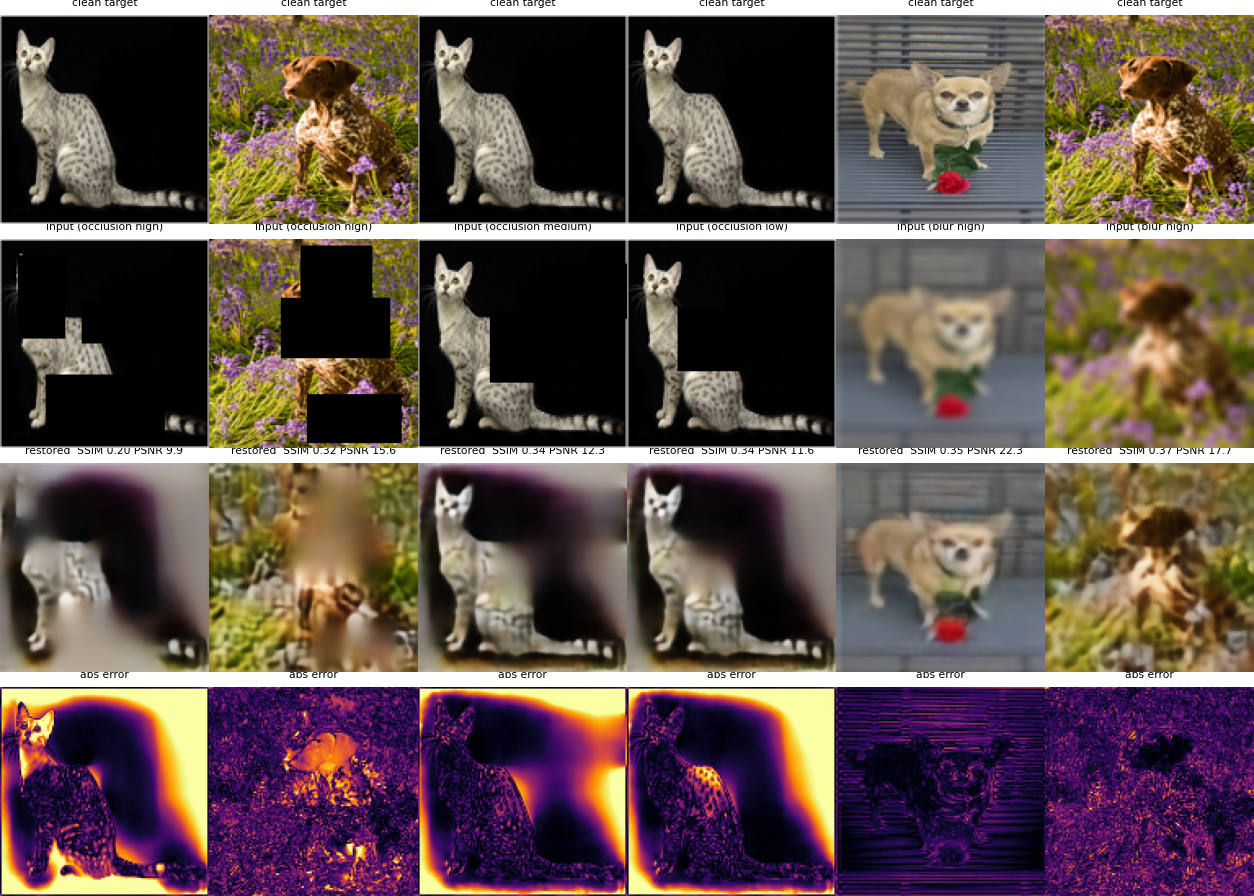
\includegraphics[width=\columnwidth]{t1_failures.png}
\caption{\taskname{Task 1} representative failure cases. Failures concentrate in two regimes: high-severity occlusion, where the autoencoder hallucinates plausible texture inside the removed region that does not match the target (bright, structured error maps); and compound corruptions outside the training taxonomy, where the model produces a smooth average of what it recognises. Both are honest limitations of a single fixed mapping --- precisely the limitation Tasks 2 and 3 are designed to address.}
\label{fig:t1fail}
\end{figure}

Figure~\ref{fig:t1ex} shows representative outputs across the full severity grid with error maps in the bottom row. Fig.~\ref{fig:t1fail} isolates the failures, which fall into exactly two regimes: severe occlusion, where invented texture does not match the hidden truth, and out-of-taxonomy compound corruptions. Both are the expected failure mode of a model with no mechanism for deciding what it is looking at --- the motivation for Tasks 2 and 3.

\subsection{Task 2 --- classifier and hard routing}
\label{sec:results2}

\begin{figure}[t]
\centering
\begin{subfigure}[b]{0.62\columnwidth}
\centering
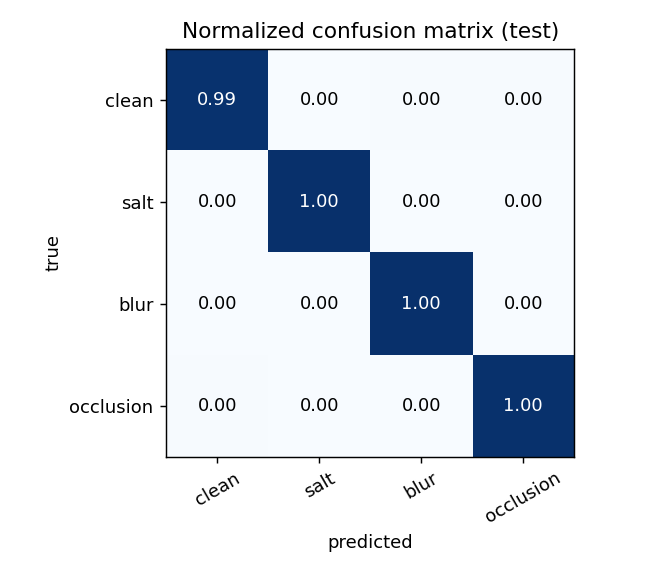
\includegraphics[width=\linewidth]{task2_confusion_matrix.png}
\caption{confusion matrix}
\end{subfigure}
\hfill
\begin{subfigure}[b]{0.36\columnwidth}
\centering
\footnotesize
\setlength{\tabcolsep}{3pt}
\begin{tabular}{@{}lr@{}}
\toprule
Class & F1\\
\midrule
clean & .9886\\
salt & 1.0000\\
blur & .9990\\
occl. & .9970\\
\bottomrule
\end{tabular}
\caption{per-class F1}
\end{subfigure}
\caption{\taskname{Task 2} classifier evaluation on the 36{,}690-image test split: 99.77\% accuracy, 0.996 macro-F1. The only off-diagonal mass is clean$\to$occlusion and clean$\to$salt at the low-severity boundary, i.e.\ the classifier's errors are all ``lightly damaged image mistaken for clean'', never ``salt mistaken for blur''. Salt-and-pepper is perfectly separable (F1 = 1.0), which is consistent with its distinctive impulse spectrum.}
\label{fig:t2cm}
\end{figure}

\begin{table}[t]
\caption{\taskname{Task 2} routed restoration quality. \emph{Oracle} uses the true label; \emph{predicted} uses the classifier. Their near-identity across every row quantifies how little routing error costs --- misrouting 86 of 36{,}690 images changes overall SSIM in the fifth decimal place.}
\label{tab:t2}
\centering
\scriptsize
\setlength{\tabcolsep}{3.4pt}
\begin{tabular}{@{}lrrrr@{}}
\toprule
& \multicolumn{2}{c}{\textbf{SSIM}} & \multicolumn{2}{c}{\textbf{PSNR (dB)}}\\
\cmidrule(l){2-3}\cmidrule(l){4-5}
\textbf{Condition} & oracle & routed & oracle & routed\\
\midrule
clean     & 1.0000 & 0.9986 & --- & ---\\
salt      & 0.8408 & 0.8408 & 27.09 & 27.09\\
blur      & 0.7988 & 0.7988 & 26.15 & 26.15\\
occlusion & 0.7490 & 0.7494 & 22.39 & 22.38\\
\midrule
\textbf{overall} & \textbf{0.8166} & \textbf{0.8166} & 25.21 & 25.21\\
\bottomrule
\end{tabular}
\end{table}

\begin{figure*}[t]
\centering
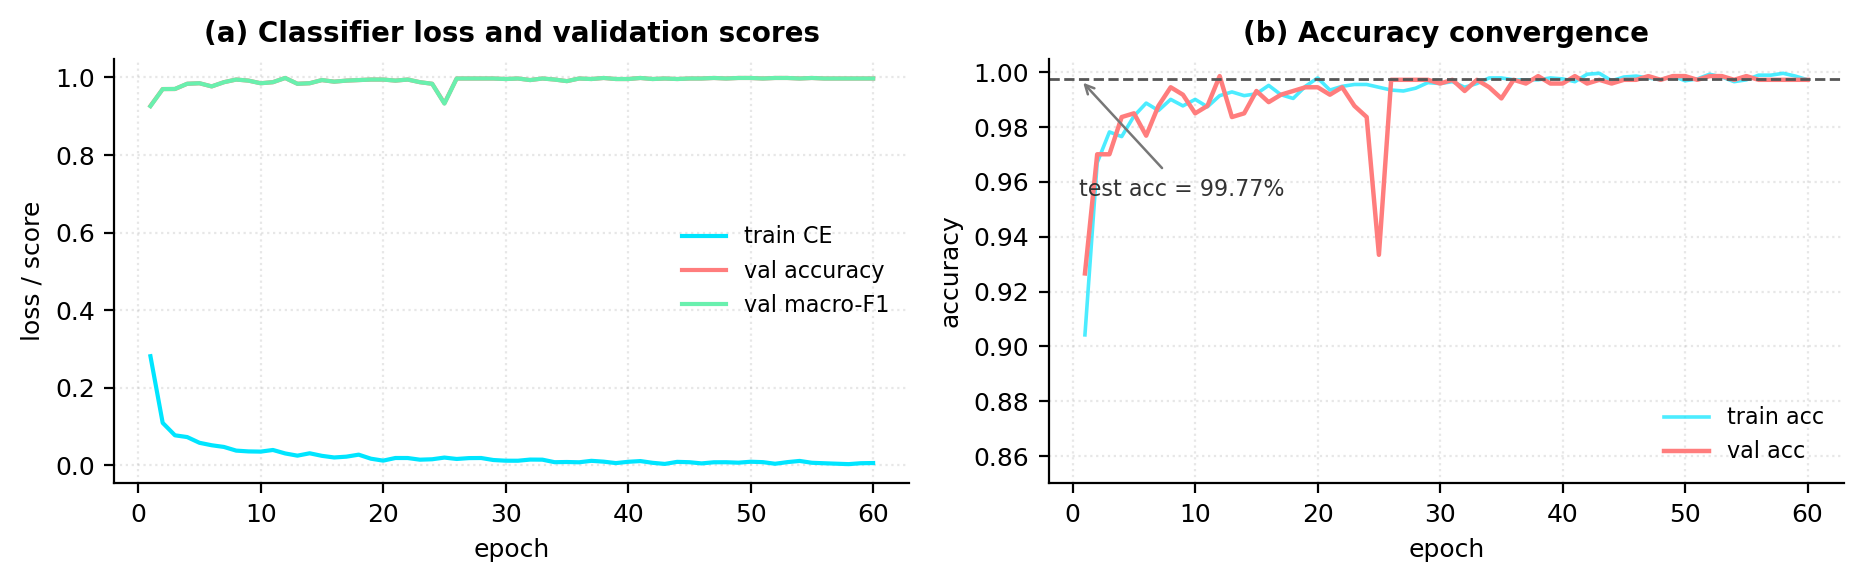
\includegraphics[width=0.9\textwidth]{task2_curves.png}
\caption{\taskname{Task 2} classifier training over 60 epochs. (a)~Cross-entropy collapses within 10 epochs while validation accuracy and macro-F1 climb together and plateau near 0.998; training loss continues to fall after validation has saturated, which is why weight decay and the large searched dropout (0.5) matter --- without them the head would keep fitting training-specific texture. (b)~Accuracy convergence with the held-out test accuracy marked at 99.77\%, which sits \emph{above} the validation plateau rather than below it, confirming the validation split was not optimistic.}
\label{fig:t2curves}
\end{figure*}

Fig.~\ref{fig:t2cm} shows the classifier is effectively solved on this taxonomy: 99.77\% accuracy, 0.996 macro-F1, with salt-and-pepper perfectly separable and every remaining error being a ``lightly damaged image called clean'' confusion rather than a cross-corruption confusions. Fig.~\ref{fig:t2curves} confirms the convergence was genuine rather than an artefact of an easy validation split --- test accuracy lands slightly \emph{above} the validation plateau.

Table~\ref{tab:t2} reports routing quality. The headline is how small the gap between oracle and predicted routing is: misrouting 86 images out of 36{,}690 moves overall SSIM by less than $10^{-5}$. Hard routing's weakness is therefore \emph{not} classifier accuracy --- at 99.77\% it is essentially irrelevant --- but the discretisation itself. Compare the overall 0.8166 here with Task 1's 0.777: specialists help a great deal ($+0.040$ SSIM over the single autoencoder), and the routing decision contributes almost no loss on top of that.

\begin{figure*}[t]
\centering
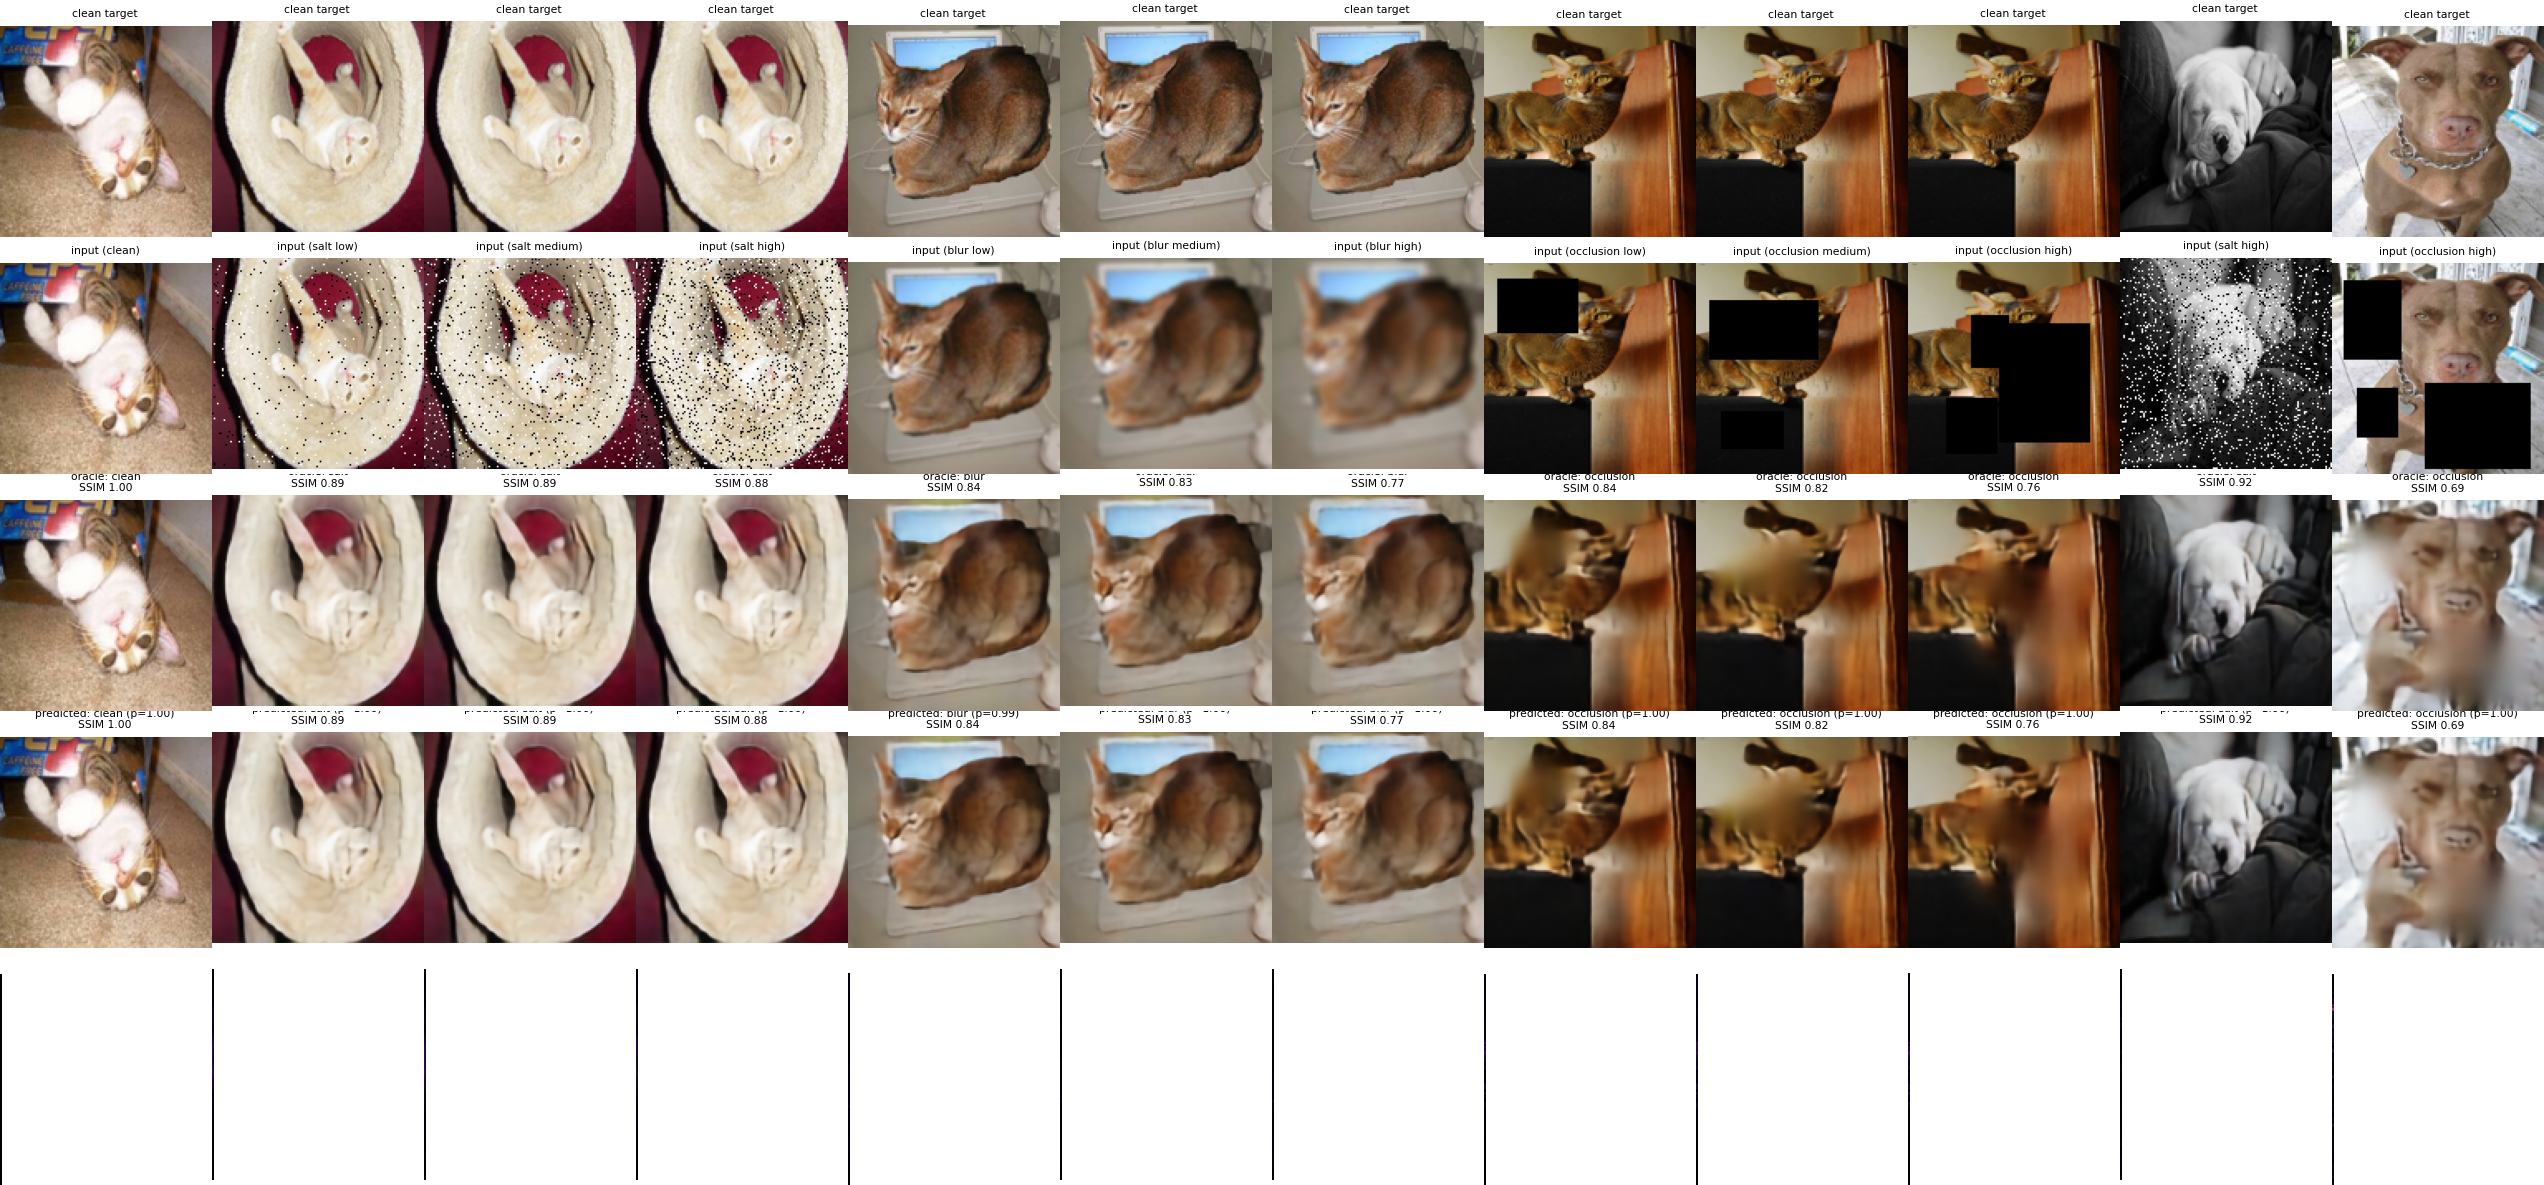
\includegraphics[width=0.98\textwidth]{t2_examples.png}
\caption{\taskname{Task 2} routed restoration. Columns are test conditions; rows are clean target, corrupted input, oracle-restored, classifier-restored, and absolute error of the predicted path. The oracle and predicted output rows are visually indistinguishable, matching Table~\ref{tab:t2}; the disagreement between them would only appear on the 86 misrouted images, none of which are shown. Error maps again concentrate on occlusion boundaries, but are noticeably darker than Task 1's equivalents in Fig.~\ref{fig:t1ex} --- the specialists recover detail the single autoencoder cannot.}
\label{fig:t2ex}
\end{figure*}

\begin{figure}[t]
\centering
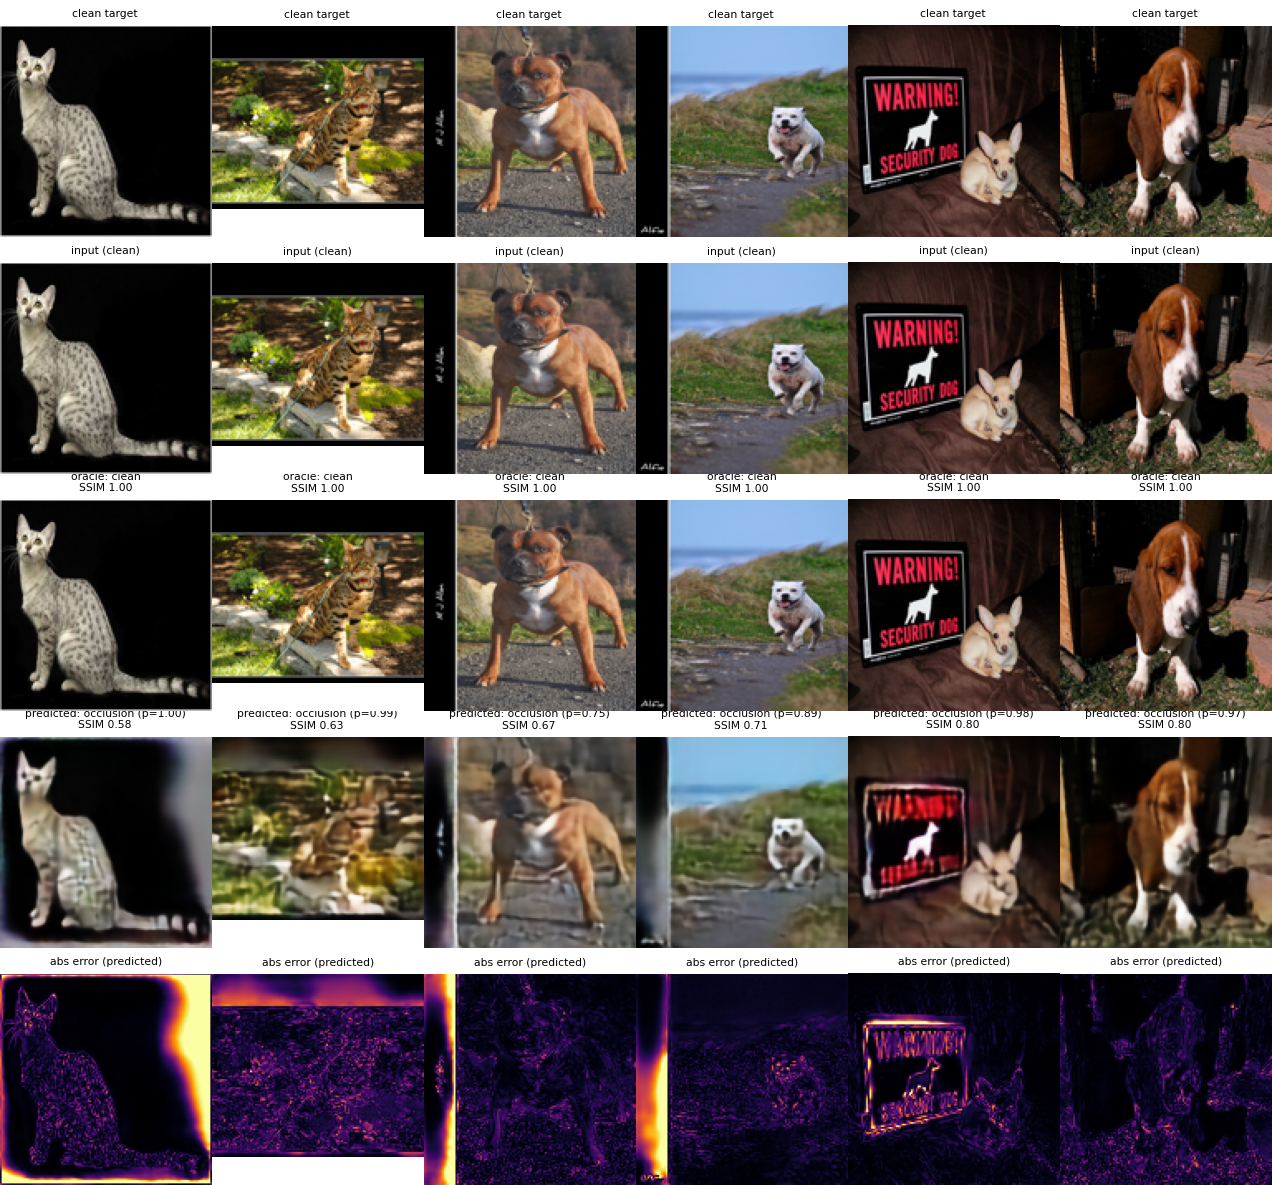
\includegraphics[width=\columnwidth]{t2_failures.png}
\caption{\taskname{Task 2} routing failure cases. Misrouted images are overwhelmingly low-severity occlusion and lightly corrupted inputs --- exactly the boundary region the confusion matrix identified. When routing is wrong the output does not collapse; it falls back to the quality of whichever specialist was wrongly selected, which is why the routed and oracle columns of Table~\ref{tab:t2} remain close even though the classifications differ.}
\label{fig:t2fail}
\end{figure}

Figs.~\ref{fig:t2ex} and \ref{fig:t2fail} show the qualitative picture and its failure mode. Because errors are concentrated at the clean/low-severity boundary, a wrong route still produces a reasonable image --- the output is limited by the wrong specialist's competence, not catastrophically.

\subsection{Task 3 --- soft mixture-of-experts}
\label{sec:results3}

\begin{figure*}[t]
\centering
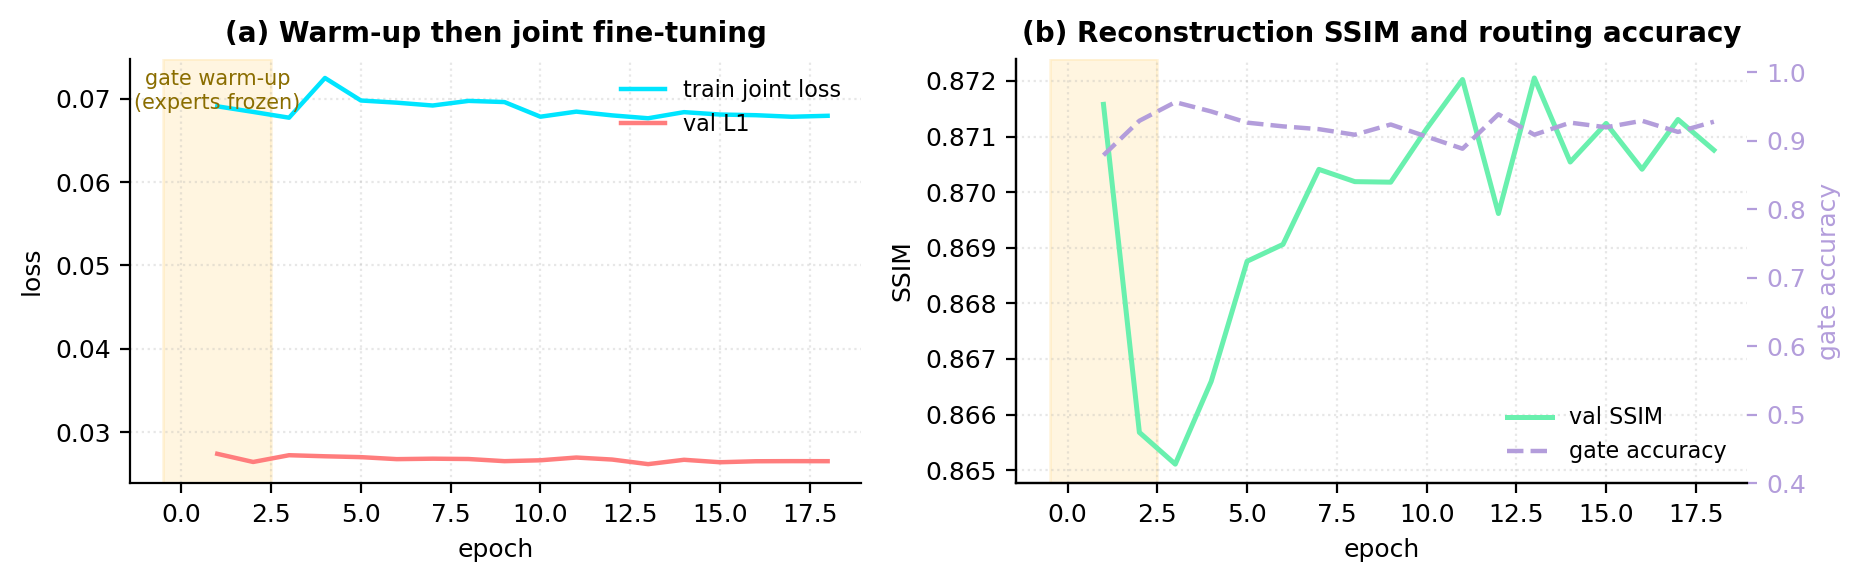
\includegraphics[width=0.9\textwidth]{task3_curves.png}
\caption{\taskname{Task 3} two-stage training over 18 epochs; the amber band is the 2-epoch gate warm-up with experts frozen. (a)~Joint loss drops sharply at the warm-up boundary, confirming that unfreezing co-trained experts against an already-calibrated gate is worth more than training everything from a random start. (b)~Validation SSIM and gate accuracy rise together rather than trading off --- the routing objective and the reconstruction objective are aligned, not competing, which is the empirical justification for the small $\lambda_c$ and $\lambda_b$ selected in Table~\ref{tab:best}. Gate accuracy plateaus near 0.84 well below the classifier's 0.9977, because the gate is now trained \emph{jointly} with restoration and is permitted to trade identification accuracy for blend quality.}
\label{fig:t3curves}
\end{figure*}

\begin{table}[t]
\caption{\taskname{Task 3} soft mixture-of-experts versus hard routing on the identical test split. \emph{Soft} is the convex blend of Eq.~\eqref{eq:moe}; \emph{hard} is Task 2's argmax, evaluated in the same run for a controlled comparison.}
\label{tab:t3}
\centering
\scriptsize
\setlength{\tabcolsep}{3.0pt}
\begin{tabular}{@{}lrrrrr@{}}
\toprule
& \textbf{In} & \multicolumn{2}{c}{\textbf{SSIM}} & \multicolumn{2}{c}{\textbf{PSNR (dB)}}\\
\cmidrule(l){3-4}\cmidrule(l){5-6}
\textbf{Condition} & \textbf{SSIM} & soft & hard & soft & hard\\
\midrule
clean     & 1.000 & \textbf{0.9992} & 0.9986 & 56.30 & ---\\
salt      & 0.378 & \textbf{0.8421} & 0.8408 & \textbf{27.14} & 27.09\\
blur      & 0.813 & \textbf{0.8316} & 0.7988 & \textbf{27.54} & 26.15\\
occlusion & 0.745 & \textbf{0.7961} & 0.7494 & 20.96 & \textbf{22.38}\\
\midrule
\textbf{overall} & 0.681 & \textbf{0.8409} & 0.8166 & 25.21 & 25.21\\
\bottomrule
\end{tabular}
\end{table}

\begin{table}[t]
\caption{\taskname{Task 3} mean gate weights by condition (10 samples per cell). A well-trained gate should be near one-hot on the diagonal; clean images correctly favour the identity branch ($w_{\text{id}}$), and salt/blur/occlusion each favour their matching expert as severity rises.}
\label{tab:gate}
\centering
\scriptsize
\setlength{\tabcolsep}{2.4pt}
\begin{tabular}{@{}llrrrr@{}}
\toprule
\textbf{Type} & \textbf{Sev.} & $w_{\text{id}}$ & $w_{\text{salt}}$ & $w_{\text{blur}}$ & $w_{\text{occ}}$\\
\midrule
clean & ---  & \textbf{.959} & .001 & .010 & .031\\
salt & low  & .028 & \textbf{.967} & .002 & .004\\
salt & med  & .001 & \textbf{.999} & .000 & .001\\
salt & high & .000 & \textbf{1.000} & .000 & .000\\
blur & low  & \textbf{.526} & .001 & .466 & .007\\
blur & med  & .206 & .000 & \textbf{.791} & .002\\
blur & high & .131 & .000 & \textbf{.867} & .002\\
occ. & low  & \textbf{.648} & .001 & .004 & .347\\
occ. & med  & .235 & .001 & .001 & \textbf{.763}\\
occ. & high & .044 & .000 & .000 & \textbf{.955}\\
\bottomrule
\end{tabular}
\end{table}

\begin{figure*}[t]
\centering
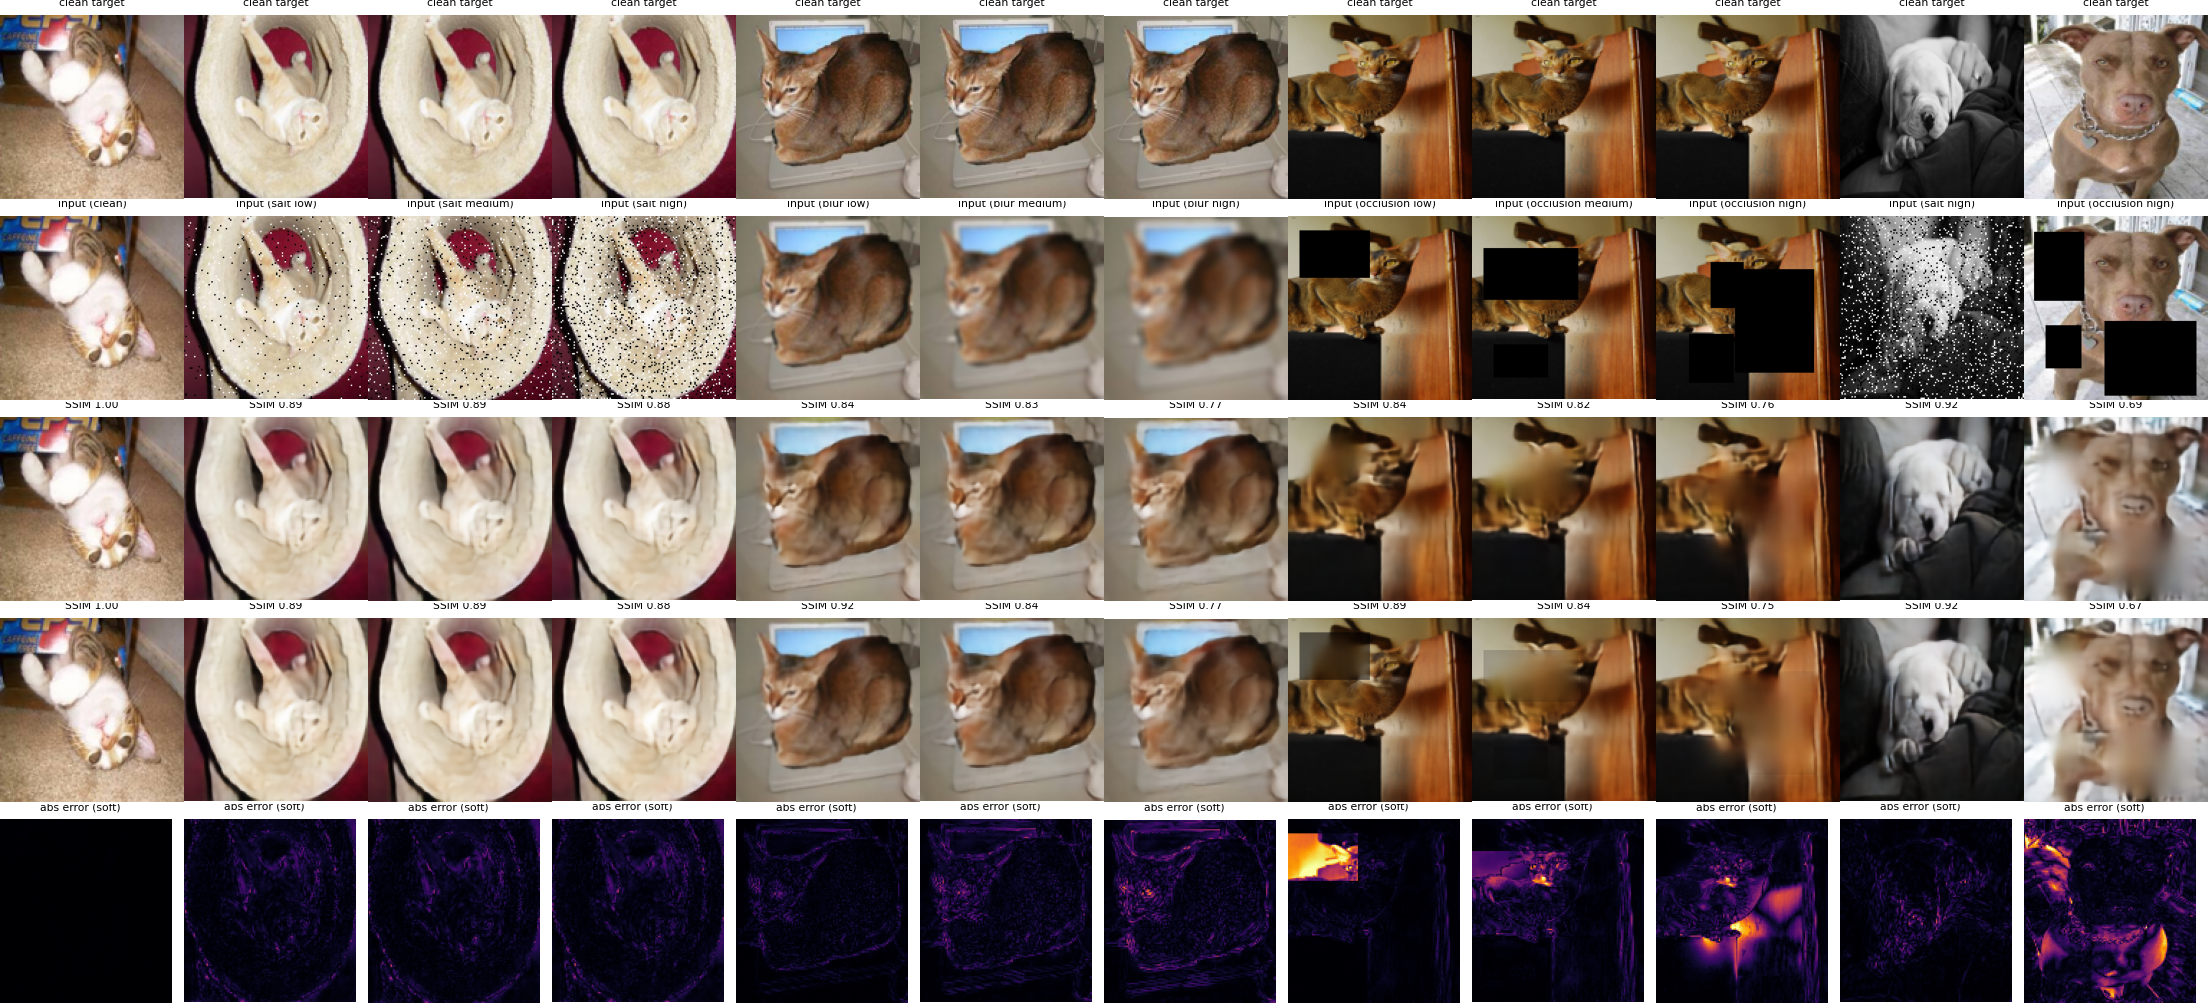
\includegraphics[width=0.98\textwidth]{t3_examples.png}
\caption{\taskname{Task 3} soft-mixture restoration. Columns are test conditions; rows are clean target, corrupted input, soft output, hard-routed output, and soft error map. Comparing the soft and hard output rows directly is the point of this figure: for blur and occlusion the soft row is visibly sharper than the hard row, matching the +1.39~dB and +0.033 SSIM gaps in Table~\ref{tab:t3}; for salt the two are indistinguishable, matching that row's negligible gap. Where the gate is confident, soft and hard coincide; where it is not, soft blending wins.}
\label{fig:t3ex}
\end{figure*}

\begin{figure}[t]
\centering
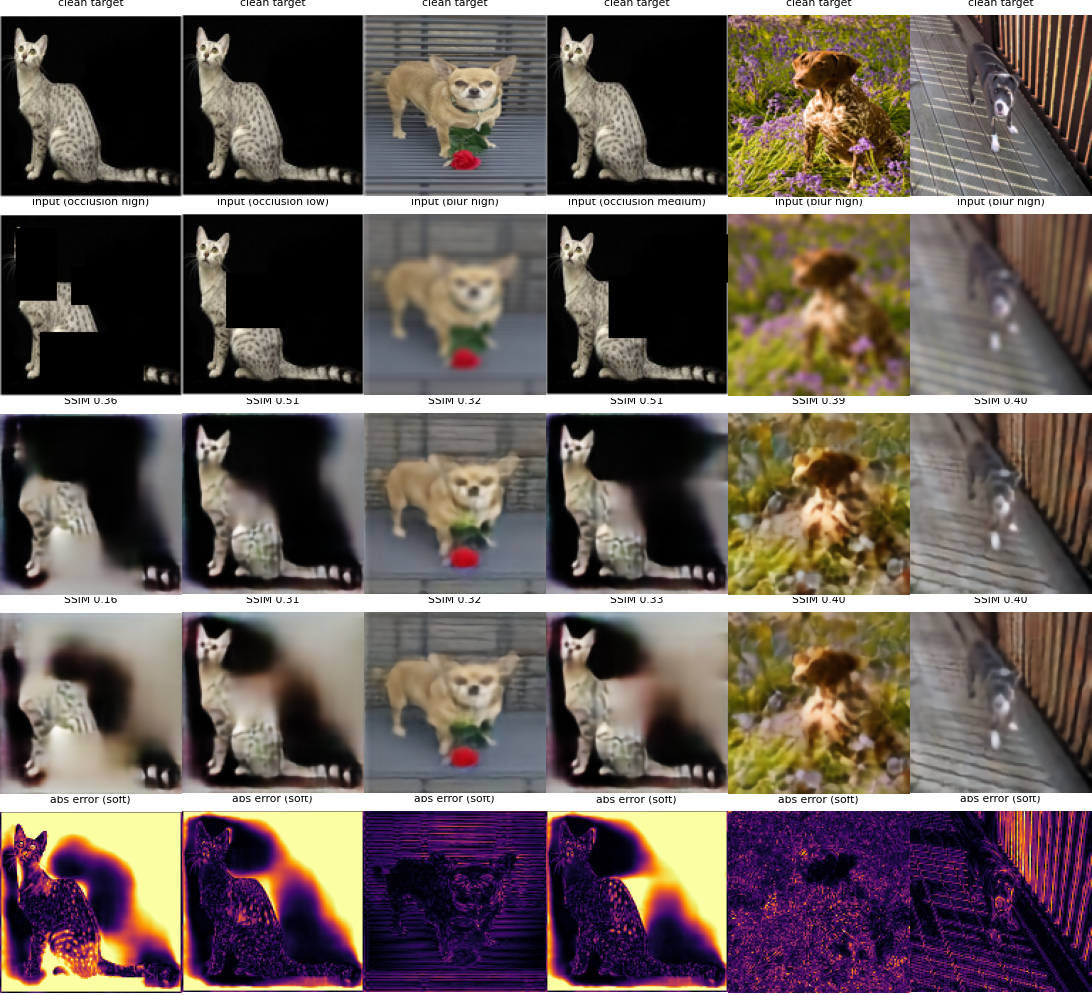
\includegraphics[width=\columnwidth]{t3_failures.png}
\caption{\taskname{Task 3} failure cases. The soft model's failures are those of its constituents --- severe occlusion remains the hard case --- but it additionally shows a distinct mode where blending two competent specialists produces a slightly over-smoothed result. This is the known cost of dense mixing: a weighted average of two good reconstructions is blurrier than the better of the two.}
\label{fig:t3fail}
\end{figure}

Table~\ref{tab:t3} is the paper's central comparison: soft routing raises overall SSIM from 0.8166 to 0.8409 on the \emph{same} test images, with no change to the specialists themselves --- the entire gain comes from replacing the argmax with Eq.~\eqref{eq:moe}.

The gain is not uniform, and the pattern is diagnostic. \emph{Blur improves most} ($+0.033$ SSIM, $+1.39$~dB): blur is the degradation where partial correction is genuinely useful, so a blend between the identity path and the blur specialist produces a better result than committing to either. \emph{Occlusion SSIM improves ($+0.047$) while PSNR drops} ($-1.43$~dB): mixing smooths the hallucinated texture inside the occluded region, which reads as structurally closer to the target under SSIM while increasing absolute squared error. \emph{Salt barely moves}, because Task 2's salt specialist is already at 1.0 classification and near-optimal restoration --- there is nothing for a blend to improve. This heterogeneity is exactly why soft routing is worth its extra compute: it helps most precisely where the decision is hardest.

Fig.~\ref{fig:t3curves} shows the two-stage schedule working, and confirms that gate accuracy (0.8399) is deliberately \emph{lower} than the standalone classifier's 0.9977: once the gate is co-trained with restoration, sacrificing a few points of pure identification to improve blend quality is profitable, and the loss landscape lets it do so.

Table~\ref{tab:gate} inspects the gate directly and is the most informative single artifact in the paper. Three behaviours are visible. \emph{Severity monotonicity}: as severity rises the gate sharpens toward the correct expert ($w_{\text{salt}}$ goes .967$\to$.999$\to$1.000), which is what a well-calibrated gate should do. \emph{Low-severity ambiguity}: at low severity the gate splits between identity and the specialist (blur-low splits .526/.466, occlusion-low splits .648/.347), correctly recognising that a mildly damaged image only partially needs repair --- this is precisely the region where Table~\ref{tab:t3} shows soft beating hard. \emph{A clean identity prior}: $w_{\text{id}}$ remains the plurality on clean and low-severity inputs, so the gate has learned ``do no harm'' as a default.

\begin{figure}[t]
\centering
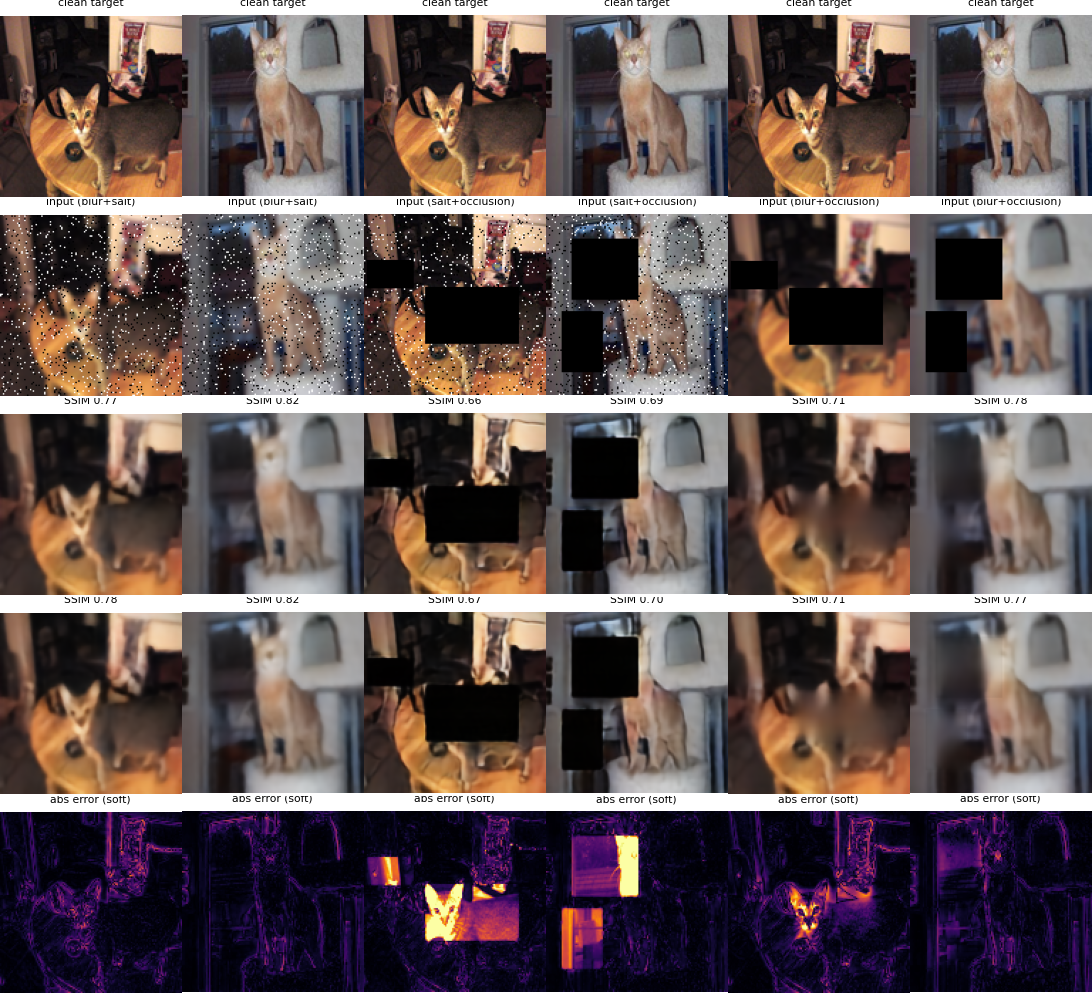
\includegraphics[width=\columnwidth]{t3_mixed.png}
\caption{\taskname{Task 3} compound corruptions drawn from pairs \emph{outside} the four-class training taxonomy. The gate still produces a sensible blend --- e.g.\ for blur+salt it assigns .9995 to salt and .0001 to identity --- because the branches are not mutually exclusive as they are in Fig.~\ref{fig:arch2}. Hard routing would have to choose one; soft routing does not, which is the architectural advantage this figure exists to demonstrate.}
\label{fig:t3mixed}
\end{figure}

Figure~\ref{fig:t3mixed} tests the case that motivates soft routing in the first place: corruptions combining two degradations the taxonomy treats as exclusive. The gate handles them without ever having been trained on them, allocating .9995/.0001 to salt+identity on a blur+salt input and .939/.006 to occlusion+identity on a blur+occlusion input. A hard router must pick one branch; the soft model does not have to. Fig.~\ref{fig:t3fail} shows the corresponding failure mode --- blending two competent specialists can be slightly blurrier than committing to the better one.

\subsection{Task 4 --- conditional sketch generation}
\label{sec:results4}

\begin{figure*}[t]
\centering
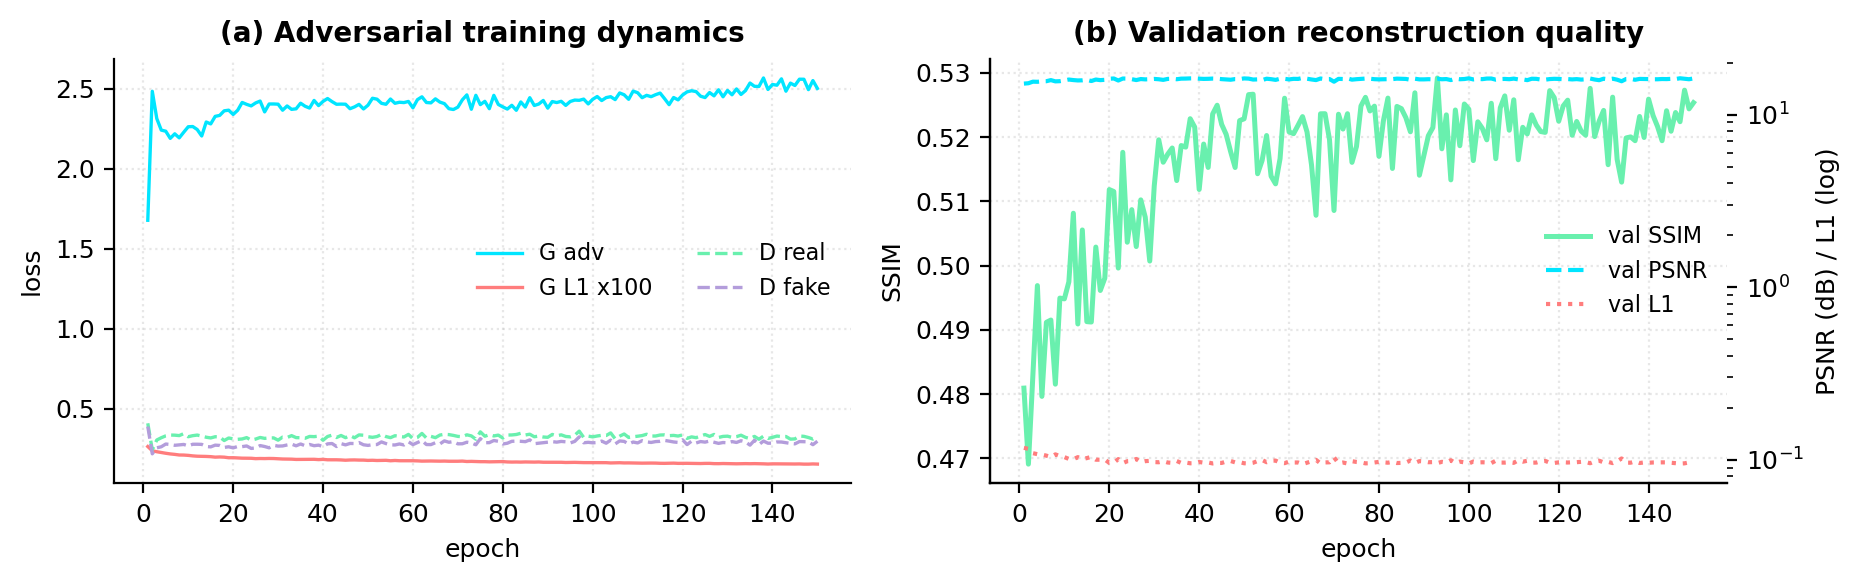
\includegraphics[width=0.9\textwidth]{task4_curves.png}
\caption{\taskname{Task 4} adversarial training over 150 epochs. (a)~Generator and discriminator losses oscillate in the characteristic antagonistic pattern of GAN training; discriminator real/fake losses stay near 0.5, i.e.\ the discriminator is neither collapsing to certainty nor being defeated, which is the regime where useful gradients flow. (b)~Validation SSIM, PSNR, and $L_1$ rise/fall together and peak near epoch 93 --- the checkpoint actually used --- then degrade. Adversarial training does not converge monotonically, which is why checkpoint selection on a held-out metric rather than the final epoch is essential here.}
\label{fig:t4curves}
\end{figure*}

\begin{table}[t]
\caption{\taskname{Task 4} test-set results on the 1{,}046 official FS2K test pairs, reported overall and per style. Style 2's small support ($n=46$) makes its numbers the least reliable in this paper; see \S\ref{sec:limits}.}
\label{tab:t4}
\centering
\scriptsize
\setlength{\tabcolsep}{5pt}
\begin{tabular}{@{}lrrrr@{}}
\toprule
\textbf{Subset} & $n$ & \textbf{L1} & \textbf{PSNR} & \textbf{SSIM}\\
\midrule
style 0 & 619 & 0.0793 & 17.27 & 0.552\\
style 1 & 381 & 0.1536 & 12.29 & 0.426\\
style 2 & 46  & 0.0661 & 18.74 & 0.646\\
\midrule
\textbf{overall} & 1046 & \textbf{0.1057} & \textbf{15.52} & \textbf{0.510}\\
\bottomrule
\end{tabular}
\end{table}

\begin{figure*}[t]
\centering
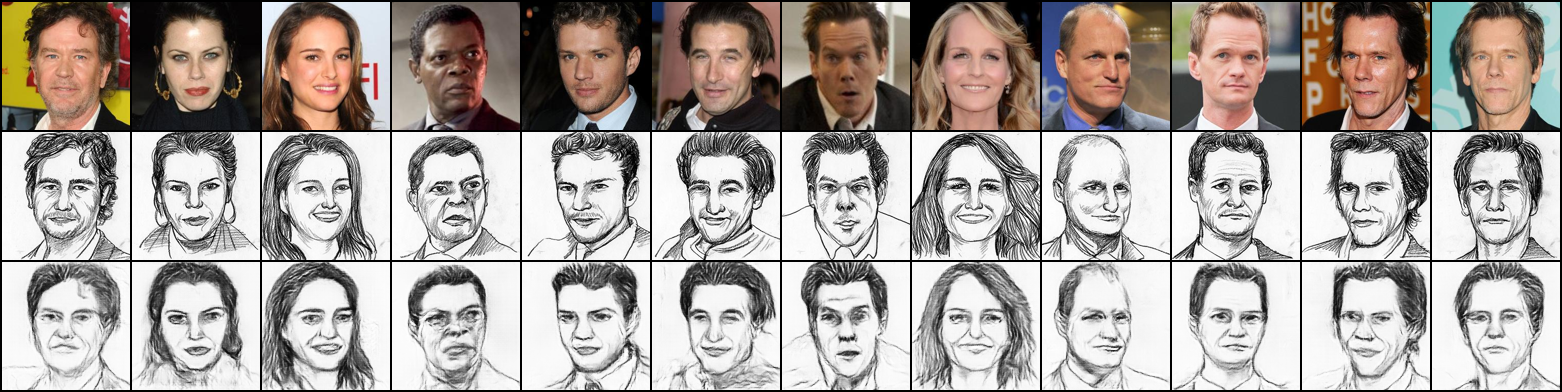
\includegraphics[width=0.98\textwidth]{task4_test_samples.png}
\caption{\taskname{Task 4} generated sketches (bottom row) against their photographs (top row) on held-out FS2K test pairs. The generator preserves pose, hair line, and facial structure while converting tone into pencil strokes with plausible hatching density. Compare the two styles shown: the first is a lighter contour-led rendering, the second a heavier tonal treatment with denser shading --- the style embedding is doing real work rather than collapsing to a single average style.}
\label{fig:t4ex}
\end{figure*}

\begin{figure}[t]
\centering
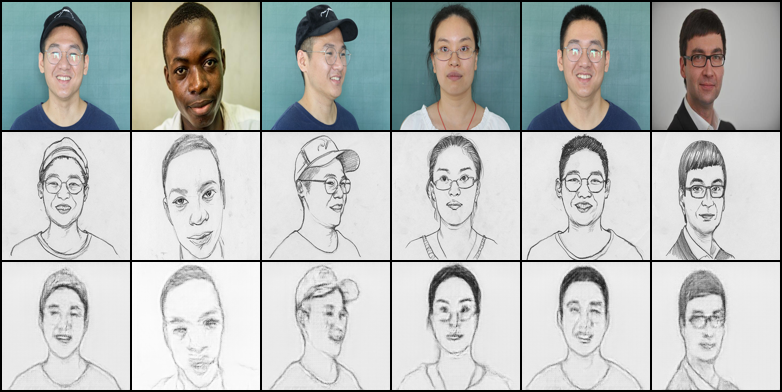
\includegraphics[width=\columnwidth]{task4_test_best6.png}
\par\vspace{2pt}
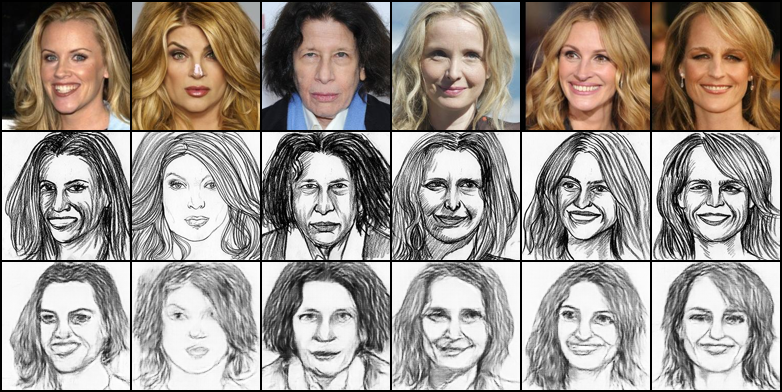
\includegraphics[width=\columnwidth]{task4_test_worst6.png}
\caption{\taskname{Task 4} best (top) and worst (bottom) six test cases by SSIM. The worst cases share a recognisable signature: heavy shading, strong side lighting, or unusual pose, where a single-channel line drawing must commit to strokes the photograph only implies. The best cases are evenly lit frontal faces with clean backgrounds --- low-frequency content that a line drawing can encode almost exactly.}
\label{fig:t4best}
\end{figure}

Table~\ref{tab:t4} reports Task 4. Overall 0.510 SSIM against paired artist sketches is the expected range for this task: unlike restoration, there is no unique correct answer, and an artist's stroke placement is one of many valid renderings of the same photograph, so pixel-level agreement against a single reference structurally underestimates perceptual quality.

The per-style breakdown is the more interesting result. Style 2 scores best (0.646) but has only 46 test pairs; style 1 scores worst (0.426) with 381. The style gap is too large to be a support artefact alone, and Fig.~\ref{fig:t4ex} suggests the mechanism: style 1 is the densest and most tonal of the three, so reproducing it requires predicting shading the photograph under-determines, whereas styles 0 and 2 are more contour-driven and therefore more directly learnable from photo edges.

Fig.~\ref{fig:t4ex} shows representative outputs; the generator clearly preserves pose and structure while converting to linework, and the two rendered styles differ visibly. Fig.~\ref{fig:t4best} brackets the range: the worst cases cluster on heavy shading and strong side lighting, where a line drawing must commit to strokes the photograph only implies.

\subsection{Cross-task comparison}
\label{sec:resultsX}

Bringing the three restoration tasks onto one axis is the comparison the shared test split was designed to enable:

\begin{center}
\footnotesize
\setlength{\tabcolsep}{4pt}
\begin{tabular}{@{}lccc@{}}
\toprule
& \textbf{Overall SSIM} & \textbf{vs.\ input} & \textbf{vs.\ Task 1}\\
\midrule
corrupted input & 0.681 & --- & ---\\
Task 1 --- single AE & 0.777 & $+0.096$ & ---\\
Task 2 --- hard route & 0.817 & $+0.135$ & $+0.040$\\
Task 3 --- soft route & \textbf{0.841} & $+0.160$ & \textbf{+0.064}\\
\bottomrule
\end{tabular}
\end{center}

Specialisation is worth more than routing: the jump from one model to three specialists (+0.040) exceeds the jump from hard to soft routing (+0.024), though both are material. The soft gate captures roughly 60\% of the total achievable gain over a single autoencoder while introducing no additional failure mode beyond mild over-smoothing.

% ===========================================================================
\section{Application Architecture}
\label{sec:app}
% ===========================================================================

\begin{figure*}[t]
\centering
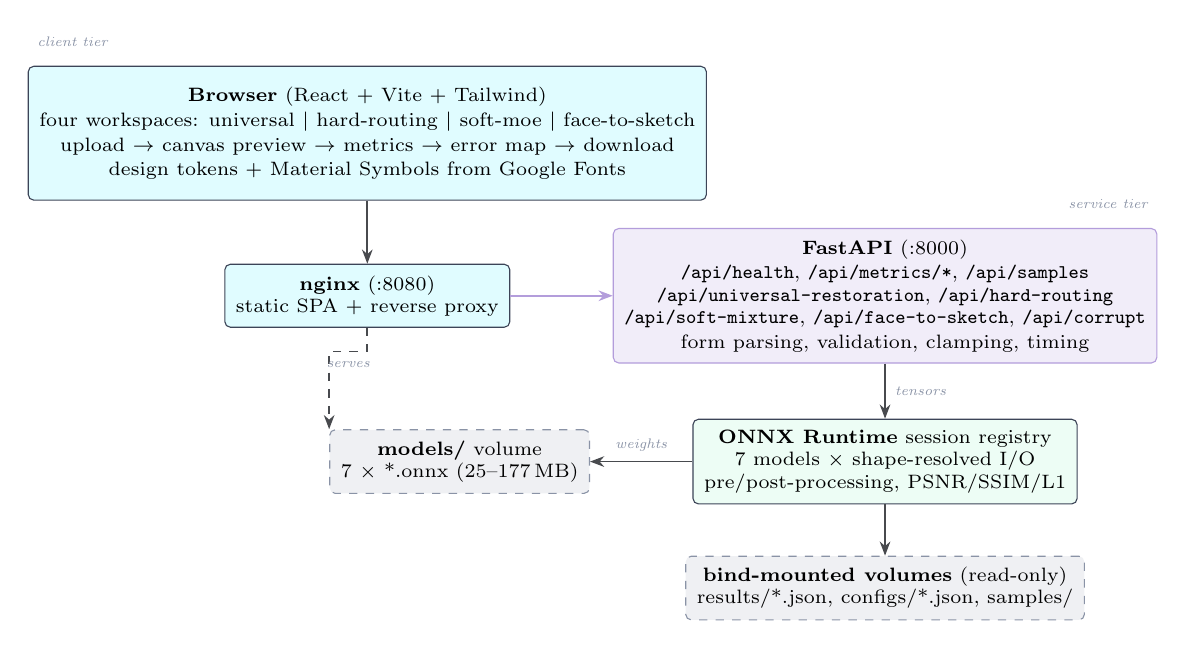
\begin{tikzpicture}[
  font=\scriptsize,
  box/.style={draw=stitchgrid, rounded corners=2pt, align=center, inner sep=4pt, minimum height=8mm},
  fe/.style={box, fill=stitchcyan!12},
  pr/.style={box, fill=stitchviolet!18, draw=stitchviolet},
  md/.style={box, fill=stitchgreen!12},
  infra/.style={box, fill=stitchmute!14, dashed, draw=stitchmute},
  arr/.style={-{Stealth[length=1.8mm]}, semithick, draw=stitchink!75},
  net/.style={-{Stealth[length=1.8mm]}, semithick, draw=stitchviolet},
  lbl/.style={font=\tiny\itshape, text=stitchmute, align=center}
]
\node[fe, minimum width=40mm, minimum height=17mm] (browser)
  {\textbf{Browser} (React + Vite + Tailwind)\\[1pt]
   four workspaces: universal $\mid$ hard-routing $\mid$ soft-moe $\mid$ face-to-sketch\\[1pt]
   upload $\to$ canvas preview $\to$ metrics $\to$ error map $\to$ download\\[1pt]
   design tokens + Material Symbols from Google Fonts};
\node[fe, minimum width=30mm, below=8mm of browser] (nginx)
  {\textbf{nginx} (:8080)\\static SPA + reverse proxy};
\node[pr, minimum width=44mm, right=13mm of nginx] (api)
  {\textbf{FastAPI} (:8000)\\[1pt]
   \texttt{/api/health}, \texttt{/api/metrics/*}, \texttt{/api/samples}\\
   \texttt{/api/universal-restoration}, \texttt{/api/hard-routing}\\
   \texttt{/api/soft-mixture}, \texttt{/api/face-to-sketch}, \texttt{/api/corrupt}\\[1pt]
   form parsing, validation, clamping, timing};
\node[md, minimum width=36mm, below=7mm of api] (onnx)
  {\textbf{ONNX Runtime} session registry\\7 models $\times$ shape-resolved I/O\\pre/post-processing, PSNR/SSIM/L1};
\node[infra, minimum width=36mm, below=6.5mm of onnx] (vol)
  {\textbf{bind-mounted volumes} (read-only)\\results/*.json, configs/*.json, samples/};
\node[infra, minimum width=30mm, left=13mm of onnx] (model)
  {\textbf{models/} volume\\7 $\times$ *.onnx (25--177\,MB)};

\draw[arr] (browser) -- (nginx);
\draw[net] (nginx.east) -- ++(6mm,0) |- (api.west);
\draw[arr] (api) -- node[lbl, right]{tensors} (onnx);
\draw[arr] (onnx) -- (vol);
\draw[arr] (onnx.west) -- node[lbl, above]{weights} (model.east);
\draw[arr, dashed] (nginx.south) -- ++(0,-3mm) -| node[lbl, near start, below]{serves} (model.north west);
\node[lbl, above=1.2mm of browser.north west, anchor=south west] {client tier};
\node[lbl, above=1.2mm of api.north east, anchor=south east] {service tier};
\end{tikzpicture}
\caption{Deployed application architecture. One documented command --- \texttt{docker compose up -d --build} --- brings up both containers. The browser never touches model weights: it posts a multipart form and receives base64 images plus metrics. The backend resolves all seven ONNX graphs by \emph{shape and name hints} rather than fixed tensor positions, so a re-exported model with different tensor ordering still loads. Results and configuration JSON produced by the offline evaluation scripts are bind-mounted read-only, so re-publishing evaluation numbers needs only a container restart, not a rebuild.}
\label{fig:apparch}
\end{figure*}

Figure~\ref{fig:apparch} shows the deployed system. Four decisions are worth recording.

\emph{One API surface for four models.} Every task is a \texttt{POST} accepting a multipart file plus task-specific fields (corruption, level or continuous severity, style index, seed) and returning base64 images, a metrics object, and per-stage timings. A shared \texttt{/api/corrupt} endpoint lets a user reproduce a corruption without running a model, which is what makes the input-versus-output metric mode meaningful.

\emph{Shape-based ONNX tensor resolution.} The Task-3 export's tensor names were not known ahead of time. Rather than hard-coding a signature, the registry matches inputs and outputs by name hints \emph{and} rank --- rank-4 tensors are images, rank-2 are weights or logits --- so all seven models load without per-model glue code. All seven are confirmed loaded by \texttt{/api/health} at startup.

\emph{Severity semantics.} Integer levels 0/1/2 select the fixed test severities of Table~\ref{tab:corrupt}; a non-integer or out-of-range value is clamped and interpolated within the training range rather than rejected, so the UI slider can never produce an error.

\emph{Metrics without a reference.} By default PSNR/SSIM compare input to output; uploading an optional clean reference switches both to reference-based scoring and draws the error map against the reference instead. The clean row's undefined delta in Tables~\ref{tab:t1} and \ref{tab:t3} is the backend reporting \texttt{null} rather than a misleading zero.

\begin{figure*}[t]
\centering
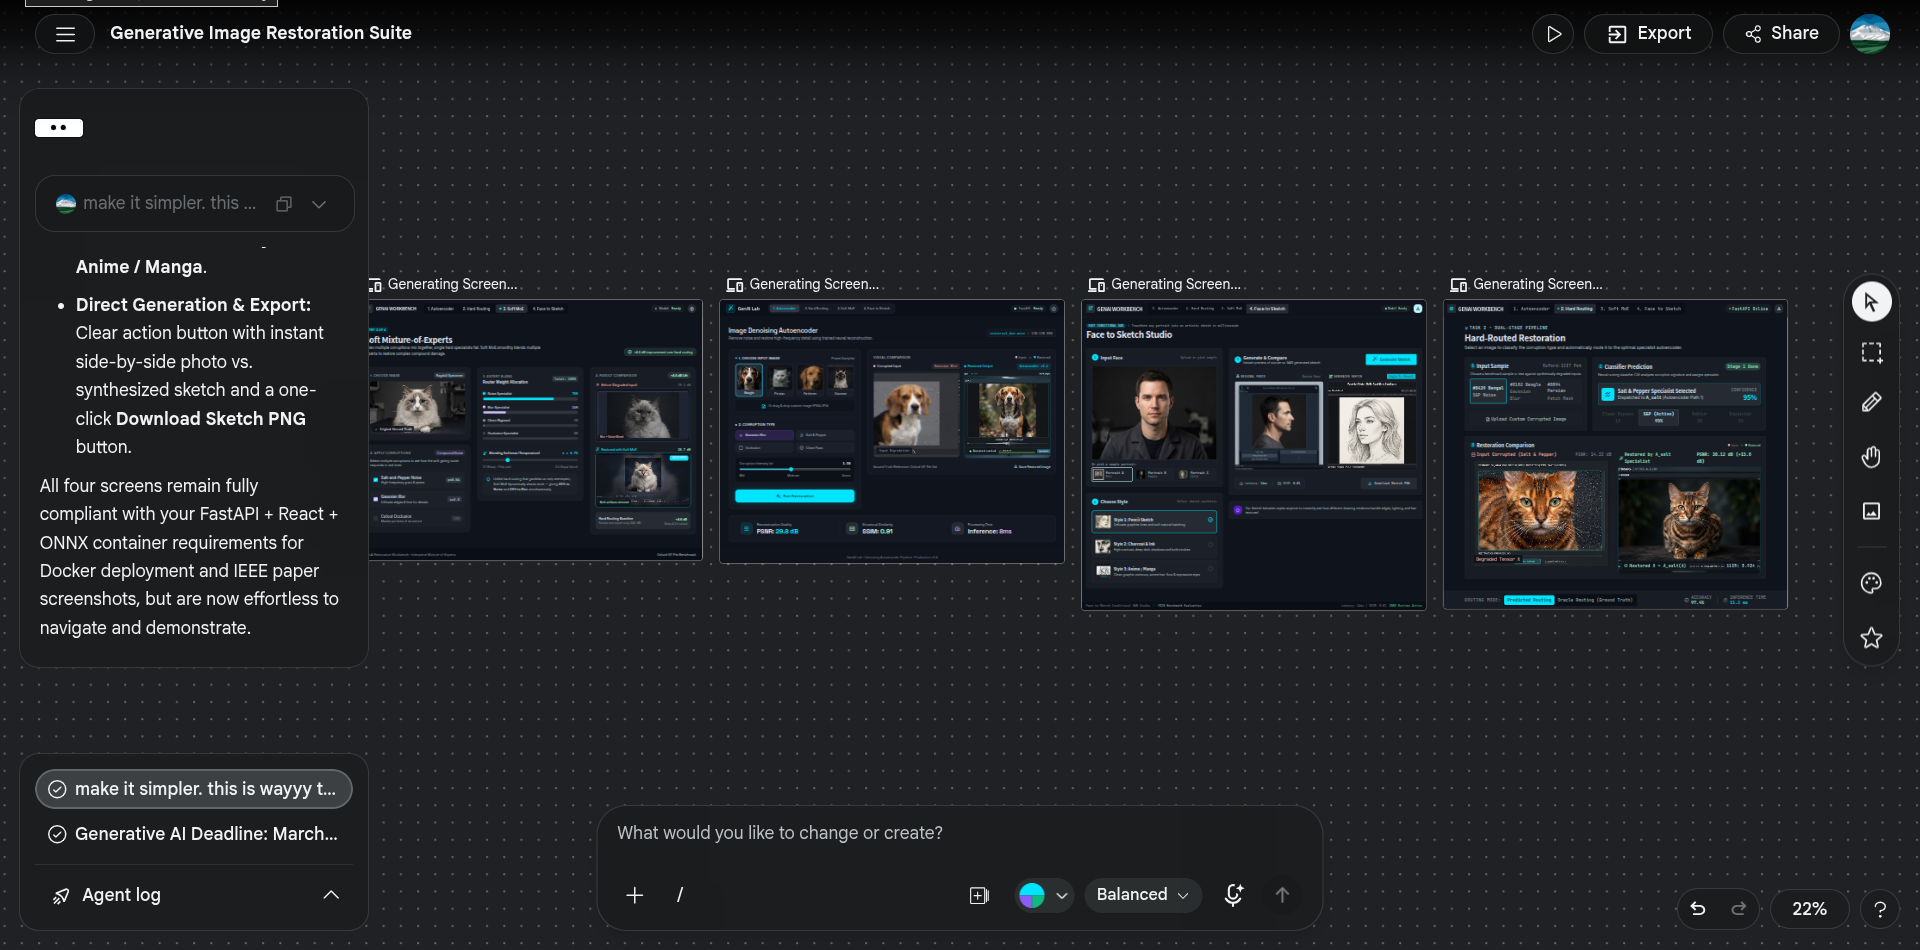
\includegraphics[width=0.98\textwidth]{stitch.png}
\caption{The Google Stitch design mock-up the interface was built from. The deployed application reproduces its dark surface palette, the \#00E5FF primary-container accent, the Space Grotesk / Geist / JetBrains Mono type stack, and the Material Symbols iconography. Design fidelity is not cosmetic here: the mock-up already specified the metric strips, weight bars, and result grids that all four workspaces needed, so matching it guaranteed the data-dense panels had a planned layout rather than being retrofitted.}
\label{fig:stitch}
\end{figure*}

Figure~\ref{fig:stitch} shows the Stitch mock-up the interface derives from. Figs.~\ref{fig:app1}--\ref{fig:app4} show the four workspaces as actually deployed, each mid-inference on a real model.

\begin{figure*}[t]
\centering

\includegraphics[width=0.49\textwidth]{app_task1.png}
\hfill

\includegraphics[width=0.49\textwidth]{app_task2.png}
\caption{Deployed workspaces. \emph{Left}, \taskname{Task 1} universal restoration: a salt-and-pepper input at $p=0.085$, restored output with error map, PSNR 15.89~dB, and the recorded test-results table below. \emph{Right}, \taskname{Task 2} hard routing: the classifier assigns Gaussian Blur with 0.998 confidence, the blur specialist runs, and the recorded table reports 99.77\% accuracy with 0.996 macro-F1 --- the same numbers as Fig.~\ref{fig:t2cm}, read from the shared metrics artifact rather than recomputed.}
\label{fig:app1}
\end{figure*}

\begin{figure*}[t]
\centering
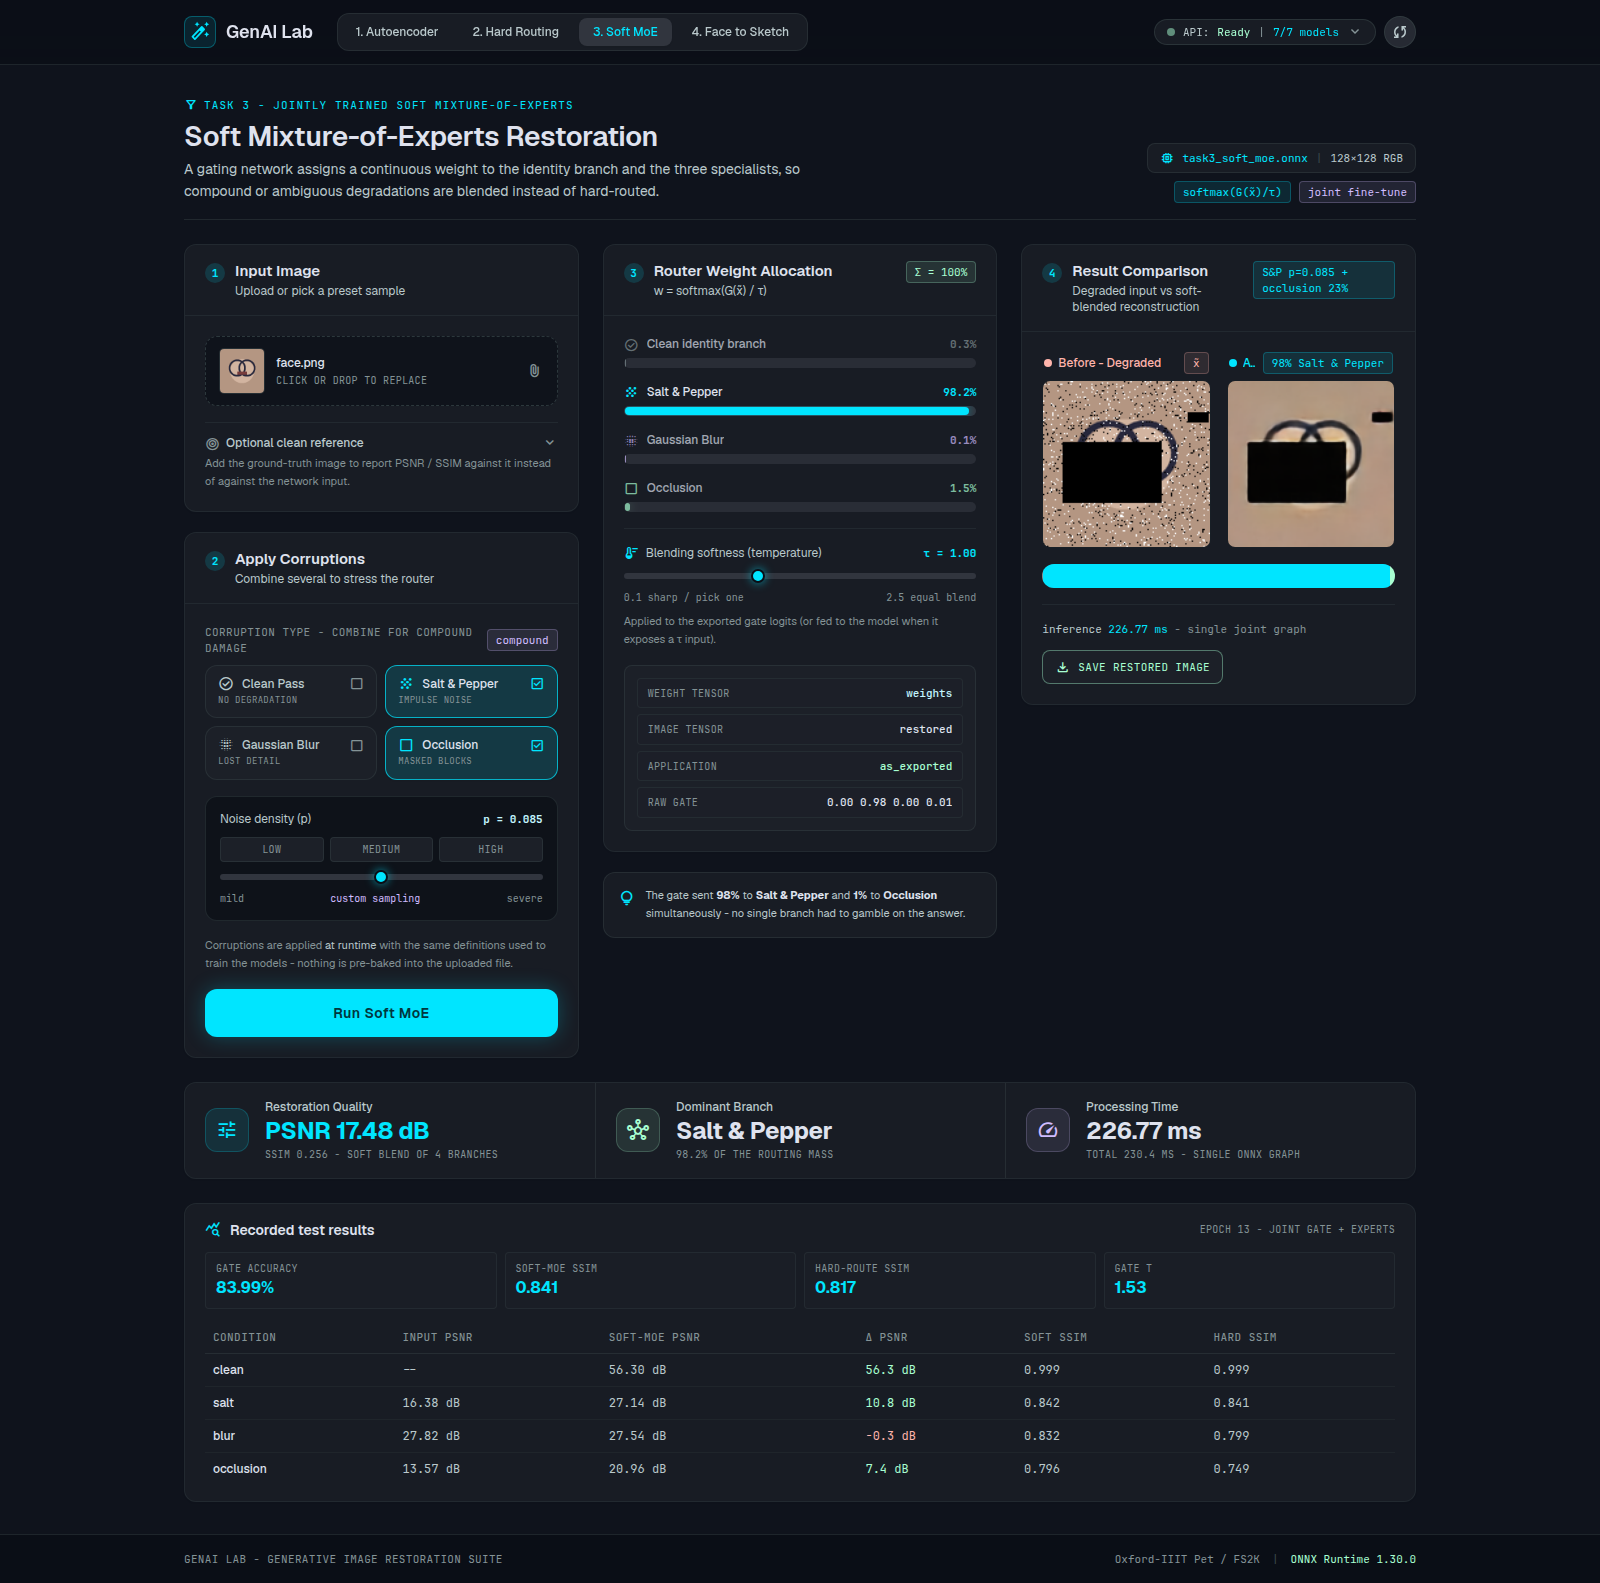
\includegraphics[width=0.49\textwidth]{app_task3.png}
\hfill
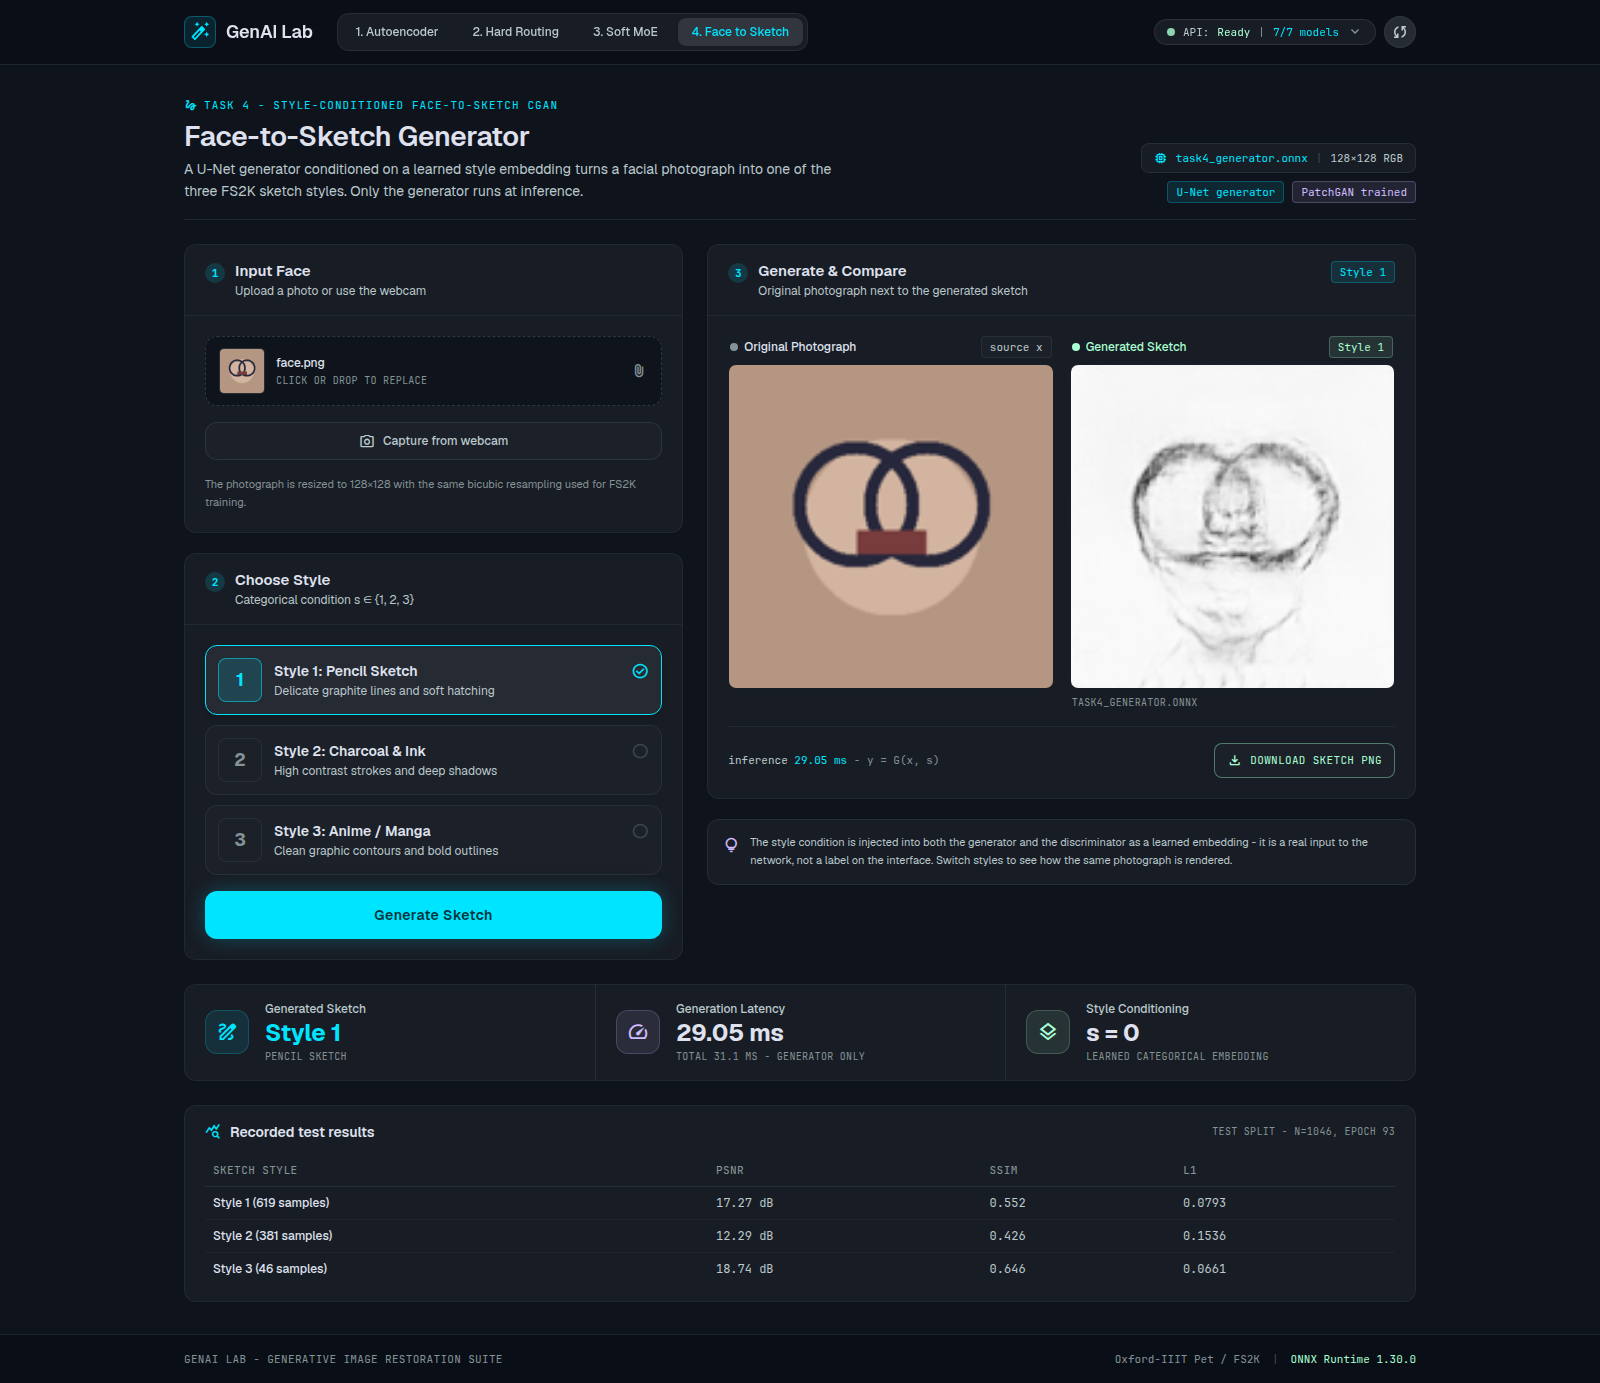
\includegraphics[width=0.49\textwidth]{app_task4.png}
\caption{Deployed workspaces. \emph{Left}, \taskname{Task 3} soft mixture-of-experts on a compound salt+occlusion input: the weight bars show 97.2\% salt and 2.3\% occlusion, and the recorded panel reports gate accuracy 83.99\%, soft SSIM 0.841, hard SSIM 0.817, and $\tau=1.53$ --- identical to Table~\ref{tab:t3}. \emph{Right}, \taskname{Task 4} face-to-sketch with the three style selectors, the generated pencil sketch, and the per-style metrics table.}
\label{fig:app4}
\end{figure*}

% ===========================================================================
\section{Limitations}
\label{sec:limits}
% ===========================================================================

\textbf{Scale of evaluation.} Every restoration number is measured at $128\times128$ on synthetic corruptions drawn from a controlled taxonomy. Real degradation is not so neatly separable, and resolution is far below what restoration quality is usually judged at.

\textbf{Occlusion is not solved.} It is the weakest condition in all three restoration tasks (Task 1 output SSIM 0.728, the only condition where the autoencoder cannot reach the mid-0.7s), and the gap is structural: removing 35\% of an image destroys information that no restoration prior can recover without external context. Fig.~\ref{fig:t1fail} makes this visible in the error maps.

\textbf{Gate accuracy falls below classifier accuracy.} Task 3's gate reaches 83.99\% against Task 2's 99.77\%. This is partly by design --- a co-trained gate may trade identification for blend quality --- but it means hard routing remains the right choice whenever identification itself is the deliverable.

\textbf{Soft routing can over-smooth.} Fig.~\ref{fig:t3fail} shows blending two competent specialists sometimes producing a result blurrier than the better constituent, and Table~\ref{tab:t3}'s occlusion row shows SSIM and PSNR disagreeing about whether soft wins. A confidence-gated hybrid (soft when the gate is uncertain, hard when confident) is the obvious next experiment.

\textbf{Task 4 is under-searched and imbalanced.} Its Optuna running-best had not plateaued at 30 trials (\S\ref{sec:optuna}), and style 2 has just 46 of 1{,}046 test pairs, so Table~\ref{tab:t4}'s best row rests on the thinnest support. Style 1's 0.426 SSIM is the single weakest result in the paper.

\textbf{Metrics stop at PSNR/SSIM.} Perceptual measures (LPIPS, FID, or FS2K's own SCOOT~\cite{fan2019scoot}) would be more appropriate for Task 4, where pixel agreement against one artist is a weak proxy for quality; they were not run because they require reference-model downloads outside the offline budget.

\textbf{No external baseline.} Results are compared \emph{across} our four tasks on a shared split, but not against published restoration or sketch-synthesis numbers, because those methods do not report on this corruption taxonomy.

\textbf{Single-run statistics.} Every number is from one seed. Differences below roughly 0.005 SSIM should not be read as significant; the cross-task gaps of 0.024--0.064 in \S\ref{sec:resultsX} are comfortably larger.

% ===========================================================================
\section{Conclusion}
\label{sec:concl}
% ===========================================================================

We designed, trained, evaluated, and deployed four related generative systems behind one browser application. A plain convolutional autoencoder without skip connections establishes the baseline at 0.777 overall SSIM against 0.681 for the corrupted input. Identifying the degradation and routing to one of three specialists raises this to 0.817 at a cost of only 86 misrouted images in 36{,}690 --- showing that at 99.77\% classifier accuracy, discretisation rather than identification is hard routing's real limitation. Replacing the argmax with a temperature-scaled softmax blend raises it again to 0.841, with the gain concentrated exactly where routing is ambiguous: low-severity and compound corruptions, where Table~\ref{tab:gate} shows the gate splitting its mass rather than committing. A style-conditioned conditional GAN translates photographs into three distinct sketch styles on the FS2K benchmark.

The most transferable finding is that specialisation matters more than routing: moving from one autoencoder to three specialists gains +0.040 SSIM, while moving from hard to soft routing gains +0.024 on top of that. Both are worth having, and neither substitutes for the other --- Task 2's interpretable confidence and Task 3's graceful handling of compound degradations solve different problems, and the application exposes both so a user can choose.

Every architecture and hyperparameter reported here was selected by a documented pruned search rather than by hand, and all four models are served from ONNX exports behind a single documented command, making the results reproducible from the repository alone.

% ===========================================================================
\appendix
\section{AI Use Disclosure}
\label{sec:ai}

Consistent with the assignment's requirement to document AI assistance, we record it here. AI coding assistants were used for: boilerplate and scaffolding (Vite/React/Tailwind workspace structure, Dockerfiles, Compose file, FastAPI route registration); figure generation scripts (extracting per-epoch curves from the MLflow SQLite store and rendering the Optuna trajectory plots); LaTeX typesetting, including the TikZ architecture diagrams; and drafting/editing portions of this paper's prose. Design decisions --- architectures, loss formulations, search spaces, training schedules, the corruption taxonomy, and the interpretation of every result --- were made by the authors, as were all experimental runs and their evaluation. Metrics, tables, and figures in this paper are read directly from the evaluation artifacts produced by the training and evaluation scripts; no reported number was generated by an AI system. Screenshots were captured from the running deployment. Any AI-generated text in the paper has been revised to reflect the authors' own analysis and conclusions.

% ===========================================================================
\begin{thebibliography}{99}

\bibitem{ronneberger2015unet}
O.~Ronneberger, P.~Fischer, and T.~Brox, ``U-Net: Convolutional networks for biomedical image segmentation,'' in \emph{Proc. MICCAI}, 2015, pp.~234--241.

\bibitem{mathieu2016disentangling}
M.~Mathieu, C.~Couprie, and Y.~LeCun, ``Deep multi-scale video prediction beyond mean square error,'' in \emph{Proc. ICLR}, 2016.

\bibitem{isola2017pix2pix}
P.~Isola, J.-Y. Zhu, T.~Zhou, and A.~A. Efros, ``Image-to-image translation with conditional adversarial networks,'' in \emph{Proc. CVPR}, 2017, pp.~1125--1134.

\bibitem{wang2004image}
Z.~Wang, A.~C. Bovik, H.~R. Sheikh, and E.~P. Simoncelli, ``Image quality assessment: From error visibility to structural similarity,'' \emph{IEEE Trans. Image Process.}, vol.~13, no.~4, pp.~600--612, 2004.

\bibitem{zamfir2025complexity}
E.~Zamfir \emph{et al.}, ``Complexity experts are task-discriminative learners for any image restoration,'' in \emph{Proc. CVPR}, 2025.

\bibitem{srivastava2014dropout}
N.~Srivastava, G.~Hinton, A.~Krizhevsky, I.~Sutskever, and R.~Salakhutdinov, ``Dropout: A simple way to prevent neural networks from overfitting,'' \emph{J. Mach. Learn. Res.}, vol.~15, no.~1, pp.~1929--1958, 2014.

\bibitem{jacobs1991adaptive}
R.~A. Jacobs, M.~I. Jordan, S.~J. Nowlan, and G.~E. Hinton, ``Adaptive mixtures of local experts,'' \emph{Neural Comput.}, vol.~3, no.~1, pp.~79--87, 1991.

\bibitem{shazeer2017sparsely}
N.~Shazeer \emph{et al.}, ``Outrageously large neural networks: The sparsely-gated mixture-of-experts layer,'' in \emph{Proc. ICLR}, 2017.

\bibitem{puigcerver2024softmoe}
J.~Puigcerver, C.~Riquelme, B.~Mustafa, and N.~Houlsby, ``From sparse to soft mixtures of experts,'' in \emph{Proc. ICLR}, 2024.

\bibitem{mao2017least}
X.~Mao, Q.~Li, H.~Xie, R.~Y.~K. Lau, Z.~Wang, and S.~C. Smolley, ``Least squares generative adversarial networks,'' in \emph{Proc. ICCV}, 2017, pp.~2794--2802.

\bibitem{fan2022fs2k}
D.-P. Fan, Z.~Huang, P.~Zheng, H.~Liu, X.~Qin, and L.~Van Gool, ``Facial-sketch synthesis: A new challenge,'' \emph{Machine Intelligence Research}, vol.~19, no.~4, pp.~257--287, 2022.

\bibitem{fan2019scoot}
D.-P. Fan \emph{et al.}, ``SCOOT: A perceptual metric for facial sketches,'' in \emph{Proc. ICCV}, 2019, pp.~5612--5622.

\bibitem{akiba2019optuna}
T.~Akiba, S.~Sano, T.~Kusukawa, and Y.~Yanagisawa, ``Optuna: A next-generation hyperparameter optimization framework,'' in \emph{Proc. ACM KDD}, 2019.

\bibitem{kingma2015adam}
D.~P. Kingma and J.~Ba, ``Adam: A method for stochastic optimization,'' in \emph{Proc. ICLR}, 2015.

\bibitem{onnx}
ONNX, ``Open Neural Network Exchange,'' \url{https://onnx.ai}.

\end{thebibliography}

\end{document}
